\documentclass[]{article}
\usepackage{amsmath}
\DeclareMathOperator\Arg{Arg}
\usepackage{amsthm}
\usepackage{amssymb}
\usepackage{ulem}
\usepackage{graphicx}
\usepackage{tikz}
\usetikzlibrary{matrix,shapes,arrows,positioning,chains}
\usepackage{tkz-base}
\usepackage{tkz-euclide}
\usepackage
[
left=2cm,
right=2cm,
top=2cm,
bottom=2cm,
]
{geometry}

\setlength\parskip{1em}

\begin{document}
	
\theoremstyle{definition}
\newtheorem{definition}{Definition}
\newtheorem{problem}{Problem}

\theoremstyle{plain}
\newtheorem{lemma}{Proposition}

\section{The binary search problem, and its variation}

Here is a git repository of a software. It is known that somewhere in the recent N commits, a bug was introduced, and the task is to efficiently find the commit that introduced the bug.

A well-known solution is to use \texttt{git bisect}, i.e. the binary search method: checking the commit at the middle of the commit list, and then depending on the result, checking the commit at the middle of one half parts of the commit list. This is the fastest method under normal conditions.

Now we make a change to the problem: if the commit to check contains the bug (i.e. it is or is after the first commit introducing the bug), the software would crash the entire computer system during the test and the tester has to reboot the computer, which takes five minutes. Testing a software without the bug still takes a short time, say, 30 seconds. In this case, what is the best way to implement the binary search?

One might want to test more ``good" commits to avoid the long time spent on ``bad" commits as much as possible. Therefore they would tend to test commits before the middle commit, resulting a test sequence ``biased" towards the earlier commits. In an extreme case, where the bad commits take forever to test, they would just test commits one by one from the earliest commit, until he finds the first commit that crashes the system. Similarly, if a bad commit actually takes less time to test, the binary search would bias towards the newer commits.

Under these conditions, the question is, using the binary search idea, what would be the best commit to test in order to minimize the time cost expectation?

\section{Mathematical formalization}

Let's formalize the question in mathematical languages:

\begin{problem}
	Given a sequence $a_0, a_1, a_2, ..., a_n$, with a number $j$ such that $a_k = 0, \forall k < j$ and $a_k = 1, \forall k \ge j$. $j$ is a random number evenly distributed among integers $1, 2, ..., n$. To get the value of $a_k$, some time is taken. The time cost is $s$ if $a_k = 0$, or $t$ if $a_k = 1$. What is the best method to find $j$ with minimal expectation of total time cost?
\end{problem}

and with some assumption clarified:
\begin{itemize}
	\item The values $a_0 = 0$ and $a_n = 1$ are already known and no need to test. Their existence in the problem is to simplify the numbering system in the solution.
	\item Testing cannot be done in parallel. One cannot start another test until the previous test is finished.
	\item Only testing takes time. Other step is assumed done instantly.
	\item One may get the result by noticing one test takes a longer time before producing the result. However, getting the result in advance does not shorten the time taken by the test, not even for the final step. The total time cost includes the final ``rebooting" time even if one already knows the answer.
\end{itemize}

\section{Testing procedure}

The binary-search-like method is illustrated in the chart below.

\tikzstyle{decision} = [diamond, draw, fill=blue!20,
text width=4.5em, text badly centered, node distance=3cm, inner sep=0pt]
\tikzstyle{block} = [rectangle, draw, fill=blue!20,
text width=5em, text centered, minimum height=4em, node distance=3cm]
\tikzstyle{line} = [draw, -latex']
\tikzstyle{cloud} = [draw, ellipse,fill=red!20, node distance=2cm,
minimum height=2em]

\begin{tikzpicture}[auto]
\node [cloud](start){start};
\node [block, below of=start](init){set $p = 0$, $q = n$};
\node [decision, below of=init](exit){$q-p = 1$?};
\node [block, below of=exit](choose){$(*)$choose integer $x$ such that $p < x < q$};
\node [decision, below of=choose](test){test $a_x$};
\node [block, left of=test](a){set $p=x$};
\node [block, right of=test](b){set $q=x$};
\node [block, right of=exit](final){set $j=q$};
\node [cloud, below of=final](end){end};

\path [line] (start) -- (init);
\path [line] (init) -- (exit);
\path [line] (exit) -- node {no} (choose);
\path [line] (choose) -- (test);
\path [line] (test) -- node {0, $+s$} (a);
\path [line] (test) -- node {1, $+t$} (b);
\path [line] (a) |-([xshift=-0.5cm,yshift=-0.5cm]a.south west)|- (exit);
\path [line] (b) |-([xshift=-0.5cm,yshift=-0.5cm]a.south west)|- (exit);
\path [line] (exit) -- node{yes} (final);
\path [line] (final) -- (end);

\end{tikzpicture}

\section{The equation}

The step $(*)$ is where we want to find the best best strategy. It can be seen that on each iteration, the algorithm is effectively solving the same problem with a smaller size where $n = p - q$, therefore we can choose x by some function $w_{s,t}(n)$ as
\[
x = w_{s,t}(p - q) + p \,,
\]
and the expectation of total time $F_{s,t}(n)$ can be expressed recursively as
\begin{equation}
F_{s,t}(n) = \frac{w}{n}(t + F_{s,t}(w)) + \frac{n-w}{n}(s + F_{s,t}(n-w))\,,
\end{equation}
where $w = w_{s,t}(n)$ represents the offset of the next testing point relative to the start of the current range. The two term represents the two possibility where the next iteration goes to the left branch or the right branch. Their probability are $\frac{w}{n}$ and $\frac{n-w}{n}$, respectively, based on the assumption of the uniform distribution of the first bad commit $j$. $t$ and $s$ are the time cost of the current iteration, and $F(...)$ is the time cost of the rest of iteration.

Our goal is to find the most efficient method, so we want to minimize the value of $F(n)$. Therefore, with an initial value $F(1) = 0$, we can define a computable function $F(n)$ over $n \in \mathbb{Z}$ as
\begin{align*}
F_{s,t}(1) &= 0\,,\\
F_{s,t}(n) &= \min_{0<w<n}^{w\in\mathbb{Z}}\left\{\frac{w}{n}(t + F_{s,t}(w)) + \frac{n-w}{n}(s + F_{s,t}(n-w))\right\} \textrm{ for } n > 1 \,.
\end{align*}


\section{Theorems}

\vspace{1cm}
\begin{definition}[Expectation function]
For parameters $s, t\in\mathbb{R}^+$ and $n \in\mathbb{Z}^+$, define
\begin{align*}
	F_{s,t}(1) &= 0\,,\\
	F_{s,t}(n) &= \min_{0<w<n}^{w\in\mathbb{Z}}\left\{\frac{w}{n}(t + F_{s,t}(w)) + \frac{n-w}{n}(s + F_{s,t}(n-w))\right\} \textrm{ for } n > 1 \,.
\end{align*}
\end{definition}

\vspace{1cm}
\begin{definition}[Cost function]
	For parameters $s, t\in\mathbb{R}^+$ and $n \in\mathbb{Z}^+$, define
	\begin{align*}
		E_{s,t}(1) &= 0\,,\\
		D^{w}_{s,t}(n) &= E_{s,t}(w) + E_{s,t}(n-w) + wt +(n-w)s,&\textrm{ for } n > 1, w=1,2,\dots,n-1, \\
		E_{s,t}(n) &= \min_{0<w<n}^{w\in\mathbb{Z}}\{D^{w}_{s,t}(n)\} &\textrm{ for } n > 1 \,,\\
		w_{s,t}(n) &= \{w \,|\, D^{w}_{s,t}(n) = E_{s,t}(n)\}\ &\textrm{ for } n > 1\,.
	\end{align*}
\end{definition}
\paragraph{Remark}
We can easily see that
\[
E_{s,t}(n) = nF_{s,t}(n)
\]
The normalized function $E(n)$ is easier to work with than $F(n)$, as it eliminates the fractional terms. More over, when $s$ and $t$ are integers, the output of $E(n)$ are as well, meaning one can program it using just integer arithmetic. From now on, we will focus on analyzing $E_{s,t}(n)$ and $w_{s,t}(n)$. Note that the optimizer $w_{s,t}(n)$ outputs a set of $w$. It is not necessarily always a single $w$ that minimize the function.


\vspace{1cm}
\begin{lemma}[Homogeneity] For any $k\in\mathbb{R}^+$ we have
\[
	E_{ks,kt}(n) = k E_{s,t}(n)
\]
\[
	w_{ks,kt}(n) = w_{s,t}(n)
\]
\end{lemma}
\begin{proof}
		Proof by induction.
	\paragraph{Base case} for $n = 1$, $E_{ks,kt}(1) = 0 = k\cdot0 = kE_{s,t}(1)$
	\paragraph{Inductive step} Assuming $E_{ks,kt}(m) = k E_{s,t}(m)$ holds for all $m = 1,2,\dots,n-1$, we can show that $E_{ks,kt}(n) = k E_{s,t}(n)$ by
	\begin{align*}
	E_{ks,kt}(n) &= \min_{w}\{E_{ks,kt}(w) + E_{ks,kt}(n-w) + wkt +(n-w)kst\}\\
	  &= \min_{w}\{k E_{s,t}(w) + k E_{s,t}(n-w) + wkt +(n-w)ks\}\\
	  &= k\min_{w}\{E_{s,t}(w) + E_{s,t}(n-w) + wt +(n-w)s\}\\
	  &=kE_{s,t}(n)
	\end{align*}
	and note that the transformation doesn't affect the choice of $w$.
\end{proof}
\paragraph{Remark}
This means it is only the ratio $s/t$ that affects the bisecting strategy.


\vspace{1cm}
\begin{lemma}[Symmetry]
	\[
		E_{s,t}(n) = E_{t,s}(n)
	\]
	\[
		w \in w_{s,t}(n) \iff n-w \in w_{t,s}(n)
	\]
\end{lemma}
\begin{proof}
	Let $w' = n - w$, we can rewrite the formula for $D^w_{s,t}(n)$ and $E_{s,t}(n)$ as
	\begin{align*}
	D^w_{s,t}(n) &= E_{s,t}(w) + E_{s,t}(n-w) + wt +(n-w)s\\
	&= E_{s,t}(n-w') + E_{s,t}(w') + (n-w')t +ws\\
	&=D^{w'}_{t,s}(n)
	\end{align*}
	\[
	E_{s,t}(n) = \min_w\{D^w_{s,t}(n)\} = \min_{w'}\{D^{w'}_{t,s}(n)\} = E_{t,s}(n)
	\]
	and the optimizer for $E_{t,s}(n)$ is the set for $w'$, consisting of all $n-w$.
\end{proof}
\paragraph{Remark}
 Together with previous proposition, this means we only needs to study either $s/t \le1$ or $s/t \ge 1$.

\vspace{1cm}
\begin{lemma}[$n$-convexity]
$E_{s,t}(n)$ as a function of $n$ is convex
\end{lemma}
\begin{lemma}[$w$-induction]
	If $w^*\in w_{s,t}(n)$, then at least one of the following is true: $w^*\in w_{s,t}(n+1)$, or $w^*+1\in w_{s,t}(n+1)$
\end{lemma}
\begin{proof}
We will prove the two properties above together using induction.

We will start using the notion of ``differential" (partial finite difference of a unit step)
\begin{align*}
\Delta_x f(x,y,\dots) &= f(x + 1,y,\dots) - f(x,y,\dots)\\
\nabla_x f(x,y,\dots) &= f(x ,y,\dots) - f(x - 1,y,\dots)
\end{align*}
The subscript $x$ indicates the variable the differential is calculated over. When the context is clear, we omit the subscript variable.

We can then formally define the convexity of $E(n)$ in terms of its differential
\[
\Delta E(n) = E(n+1) - E(n)
\]
and say that $E_{s,t}(n)$ is convex on $[1,n]$ if and only if
\[
 \Delta E(m)\le \Delta E(m+1)\quad\forall m = 1,2,\dots,n-2\quad (\text{Proposition } \mathbf{C}_n)
\]

We rephrase the $w$-induction property as
\[
w^*\in w(n) \implies w^* \in w(n+1) \lor w^*+1 \in w(n+1) \quad (\text{Proposition } \mathbf{W}_n, n\geq 2)
\]


\paragraph{Base case}
The first few values of $E(n)$ and $w(n)$ are
\begin{align*}
&E(1) = 0,\ &&\\
&E(2) = s + t, \ &&w(2) = 1,\\
&E(3) = 2s + 2t + \min\{s, t\}, \ &&w(3) = \{1\}, \{2\},\text{ or }\{1,2\}
\end{align*}
It can be seen that proposition $\mathbf{C}_1, \mathbf{C}_2, \mathbf{C}_3$ and $\mathbf{W}_2$ hold.

\paragraph{Inductive step} (a) We will show that $\mathbf{C}_n \implies \mathbf{W}_n$ for $n\ge 2$:

For a $w^*\in w(n)$, if $w^* >1$, we have
\begin{align*}
D^{w^*}(n+1) &= D^{w^*}(n) + \Delta E(n-w^*) +s\\
&\le  D^{w^* - 1}(n) + \Delta E(n-w^*) +s \quad &(\text{$D^{w^*}(n)$ is the smallest among $D^{w}(n)$})\\
&\le  D^{w^* - 1}(n) + \Delta E(n-(w^*-1)) +s \quad &(\text{Convexity $\mathbf{C}_{n}$}) \\
&=D^{w(n)-1}(n+1)
\end{align*}
On the other hand, if $w^* < n -1$, we have
\begin{align*}
D^{w^*+1}(n+1) &= D^{w^*}(n) + \Delta E(w^*) +t \\
&\le  D^{w^* + 1}(n) + \Delta E(w^*) +t \quad &(\text{$D^{w^*}(n)$ is the smallest among $D^{w}(n)$})\\
&\le  D^{w^* + 1}(n) + \Delta E(w^* + 1) +t \quad &(\text{Convexity $\mathbf{C}_{n}$}) \\
&= D^{w^*+2}(n+1)
\end{align*}
Also notice that $D^w(n+1)$ is convex over $w=1,\dots,n$ due to convexity $\mathbf{C}_{n}$. The inequalities above shows the relations about four consecutive points at the valley of the convex function:
\[
D^{w^*-1}(n+1) \ge D^{w^*}(n+1) \lesseqgtr D^{w^*+1}(n+1) \le D^{w^*+2}(n+1)
\]
(if $w^* = 1$ or $w^* = n-1$, the valley sits at either end of $D^w(n+1)$ and we can make similar deduction)

We can conclude that at least one of $D^{w^*}(n+1)$ or $D^{w^*+1}(n+1)$ is the minimum of $D^w(n+1)$, thus $\mathbf{W}_n$ holds

\vspace{0.3cm}
(b) We then show that $\mathbf{C}_{n} \land \mathbf{W}_n \land \mathbf{W}_{n-1} \implies \mathbf{C}_{n+1}$ for $n\ge 2$ :
First, notice the relation between $\Delta E$
\begin{align*}
\Delta E(n)&= \min\begin{cases}
	\Delta E(w(n)) + t \quad(w(n+1) = w(n) + 1 \text{ exists})\\
	\Delta E(n-w(n)) + s\quad(w(n+1) = w(n) \text{ exists})
\end{cases} \quad (\text{Proposition $\mathbf{W}_n$}) \\
\Delta E(n-1)&= \min\begin{cases}
\Delta E(w(n-1)) + t \quad(w(n) = w(n-1) + 1\text{ exists})\\
\Delta E(n-1-w(n-1)) + s\quad(w(n) = w(n-1)\text{ exists})
\end{cases} \quad (\text{Proposition $\mathbf{W}_{n-1}$})
\end{align*}
We can also make the following deduction
\begin{align*}
	&n > w(n)\geq w(n-1)  \text{ exists}  &(\text{Proposition $\mathbf{W}_{n-1}$})\\
	\implies& \Delta E(w(n)) + t \geq  \Delta E(w(n-1)) + t &(\text{Proposition $\mathbf{C}_n$})
\end{align*}
\begin{align*}
&n>n-w(n)\geq n-1-w(n-1)  \text{ exists}  &(\text{Proposition $\mathbf{W}_{n-1}$})\\
\implies& \Delta E(n-w(n)) + s \geq \Delta E(n-1-w(n-1)) + s &(\text{Proposition $\mathbf{C}_n$})
\end{align*}
Combining these, we get
\[
\Delta E(n)\geq \Delta E(n-1)
\]
proving proposition $\mathbf{C}_{n+1}$

\end{proof}

\vspace{1cm}
\begin{lemma}[$w$-range]
	$w_{s,t}(n)$ is always a simple integer interval $[w_{s,t}^{\min}(n), w_{s,t}^{\max}(n)]$
\end{lemma}
\begin{proof}
	This can be derived from the convexity of $D^w(n)$ over $w$
\end{proof}

\vspace{1cm}
\begin{lemma}[$w$-Lipschitz continuity]
	For $n \in \{2, 3,\dots\}$
\begin{align*}
w^{\min}_{s,t}(n+1) -  w^{\min}_{s,t}(n) &\in  \{0, 1\}\\
w^{\max}_{s,t}(n+1) - w^{\max}_{s,t}(n) &\in  \{0, 1\}
\end{align*}
\end{lemma}
\begin{proof}
	First of all, the two statements are equivalent due to the symmetry property:
	\begin{align*}
	w^{\min}_{s,t}(n+1) -  w^{\min}_{s,t}(n) = ((n+1) - w^{\max}_{t,s}(n+1)) - (n- w^{\max}_{t,s}(n)) = 1 - (w^{\max}_{t,s}(n+1) - w^{\max}_{t,s}(n))
		\end{align*}
		\begin{align*}
	w^{\min}_{s,t}(n+1) -  w^{\min}_{s,t}(n) \in  \{0, 1\} \iff w^{\max}_{t,s}(n+1) - w^{\max}_{t,s}(n) \in  \{0, 1\}
	\end{align*}
	so we can just focus on proving the first one.

	From previous properties, we know that $w^{\min}(n+1) \leq w^{\min}(n) + 1$, because otherwise there would be no value $w(n+1)$ that can be either $w^{\min}(n)$ or $w^{\min}(n) + 1$. Now we only need to prove $w^{\min}(n+1)\geq w^{\min}(n)$, or in other words, $w^{\min}(n) - 1 \notin w(n+1)$. This is obviously true for $w^{\min}(n) = 1$, so let's discuss when $w \geq 2$. We denote the differential on $D^w(n)$ as
	\[
	\Delta_w D^w(n) = D^{w+1}(n) - D^w(n)
	\]
	and we have the following differential
	\begin{align*}
	\Delta_w D^{w^{\min}(n)-1}(n) &= \Delta E(w^{\min}(n)-1) - \Delta E(n-w^{\min}(n)) + t - s\\
	\Delta_w D^{w^{\min}(n)-1}(n+1) &= \Delta E(w^{\min}(n)-1) - \Delta E(n+1-w^{\min}(n)) + t - s
	\end{align*}
	We can then deduce
	\begin{align*}
	&\Delta E(n-w^{\min}(n))\leq \Delta E(n+1-w^{\min}(n)) \quad(\text{Convexity of $E(n)$}) \\
	\implies &\Delta_w D^{w^{\min}(n)-1}(n)\geq\Delta_w D^{w^{\min}(n)-1}(n+1)
	\end{align*}
	\begin{align*}
	&\Delta_w D^{w^{\min}(n)-1}(n) < 0 \quad(\text{$w^{\min}(n)$ is the smallest minimizer})\\
	\implies &\Delta_w D^{w^{\min}(n)-1}(n+1) < 0 \\
	\implies & D^{w^{\min}(n)-1}(n+1) > D^{w^{\min}(n)}(n+1)
	\end{align*}
	This means $w^{\min}(n) -1$ can't be a minimal point of $D^{w}(n+1)$.
\end{proof}

\paragraph{Remark}
	This property provides a nice way to quickly calculate $E(n)$ for large $n$: instead of checking all $n-1$ possible values for $w$, we only need to check $w = w^{\{min,max\}}(n-1) + \{0, 1\}$ (at most 4 points)


\vspace{1cm}
\begin{lemma}[$w$-Parallelogram]
	If for some $n_{\triangleleft}$ we have
	\begin{align*}
	w_{s,t}(n_{\triangleleft}) &= \{w_{\triangleleft}\}\\
	w_{s,t}(n_{\triangleleft} + 1) &= \{w_{\triangleleft}, w_{\triangleleft} + 1\}
	\end{align*}
	then there exists $n_{\triangleright} > n_{\triangleleft} + 1$ and $w_{\triangleright} > w_{\triangleleft}$ such that
	\begin{align*}
	w_{s,t}(n_{\triangleright}) &= \{w_{\triangleright}\}\\
	\end{align*}
	and for $n = n_{\triangleleft}, n_{\triangleleft}+1,\dots,n_{\triangleright}$
	\begin{align*}
	w^{\min}_{s,t}(n) &= \max\{w_{\triangleleft}, w_{\triangleright} + n - n_{\triangleright}\}\\
	w^{\max}_{s,t}(n) &= \min\{w_{\triangleright}, w_{\triangleleft} + n - n_{\triangleleft}\}
	\end{align*}
	We will also show that
	\[
	\Delta E_{s,t}(n_{\triangleleft}) = \Delta E_{s,t}(n_{\triangleleft} + 1) = \dots \ \Delta E_{s,t}(n_{\triangleright} - 1)
	\]
\end{lemma}
\begin{proof}
	We first look at $n = n_{\triangleleft} + 1$
	\begin{align*}
	&w_{s,t}(n_{\triangleleft} + 1) = \{w_{\triangleleft}, w_{\triangleleft} + 1\} \\
	\implies& D^{w_{\triangleleft}}(n_{\triangleleft} + 1) = D^{w_{\triangleleft}+1}(n_{\triangleleft} + 1) \\
	\implies& \Delta E(w_{\triangleleft}) - \Delta E(n_{\triangleleft} - w_{\triangleleft})  = s - t
	\end{align*}
	We then look at $n = n_{\triangleleft}$. On the one hand, $w_{\triangleleft}$ is a better optimizer than its left
	\begin{align*}
	&w_{s,t}(n_{\triangleleft}) = \{w_{\triangleleft}\} \\
	\implies& D^{w_{\triangleleft}}(n_{\triangleleft}) < D^{w_{\triangleleft}-1}(n_{\triangleleft}) \\
	\implies& \Delta E(w_{\triangleleft} - 1) - \Delta E(n_{\triangleleft} - w_{\triangleleft})  < s - t
	\end{align*}
	On the other hand, $w_{\triangleleft}$ is also a better optimizer than its right
	\begin{align*}
	&w_{s,t}(n_{\triangleleft}) = \{w_{\triangleleft}\} \\
	\implies& D^{w_{\triangleleft}}(n_{\triangleleft}) < D^{w_{\triangleleft}+1}(n_{\triangleleft}) \\
	\implies& \Delta E(w_{\triangleleft} ) - \Delta E(n_{\triangleleft} - w_{\triangleleft}-1) > s - t
	\end{align*}
	The three inequalities together give
	\begin{align*}
	\Delta E(w_{\triangleleft}) &> \Delta E(w_{\triangleleft} - 1)\\
	 \Delta E(n_{\triangleleft} - w_{\triangleleft}) & >  \Delta E(n_{\triangleleft} - w_{\triangleleft}-1)
	\end{align*}
	Let $a = \Delta E(w_{\triangleleft})$, and $b = \Delta E(n_{\triangleleft} - w_{\triangleleft})$, and we can say that there exists two positive integers $p$ and $q$ such that
	\begin{align*}
	\Delta E(w_{\triangleleft}-1) &< \Delta E(w_{\triangleleft}) = \Delta E(w_{\triangleleft}+1) = \dots &= \Delta E(w_{\triangleleft}+p-1) &= a < \Delta E(w_{\triangleleft}+p) \\
	\Delta E(n_{\triangleleft} - w_{\triangleleft}-1) &< \Delta E(n_{\triangleleft} - w_{\triangleleft}) = \Delta E(n_{\triangleleft} - w_{\triangleleft} + 1) = \dots &= \Delta E(n_{\triangleleft} - w_{\triangleleft} + q - 1) &= b < \Delta E(n_{\triangleleft} - w_{\triangleleft} + q )
	\end{align*}
	This is saying that $n = w_{\triangleleft}$ starts a linear segment of length $p$ with slope $a$, and similarly $n = n_{\triangleleft} - w_{\triangleleft}$ starts a linear segment of length $q$ with slope $b$. Note that we didn't specify the value of $p$ or $q$, and they can be as small as 1. We are guaranteed that $p$ and $q$ are finite, because neither  $\Delta E(w_{\triangleleft})$ or $\Delta E(n_{\triangleleft} - w_{\triangleleft})$ can be equal to $\Delta E(n_{\triangleleft})$ (thus giving an upper bound to $p$ and $q$):
	\[
	\Delta E(n_{\triangleleft}) = \Delta E(w_{\triangleleft}) + t = \Delta E(n_{\triangleleft} - w_{\triangleleft}) + s
	\]

	Let
	\begin{align*}
	n_{\triangleright} &= n_{\triangleleft} + p + q\\
	w_{\triangleright} &= w_{\triangleleft} + p
	\end{align*}
	Let's show that $w_{s,t}(n_{\triangleright}) = \{w_{\triangleright}\}$. Consider the differential of $D^w(n_{\triangleright})$ at $w_{\triangleright}$ on both sides
	\begin{align*}
	\Delta_w D^{w_{\triangleright} - 1}(n_{\triangleright}) &= \Delta E(w_{\triangleright} - 1) - \Delta E(n_{\triangleright} - w_{\triangleright}) +t - w \\
	&=\Delta E(w_{\triangleleft} + p - 1) - \Delta E(n_{\triangleleft} - w_{\triangleleft} + q) +t - s\\
	&<a - b + t - s = 0\\
	\Delta_w D^{w_{\triangleright}}(n_{\triangleright}) &= \Delta E(w_{\triangleright}) - \Delta E(n_{\triangleright} - w_{\triangleright} - 1) +t - w \\
	&=\Delta E(w_{\triangleleft} + p) - \Delta E(n_{\triangleleft} - w_{\triangleleft} + q - 1) +t - s\\
	& > a - b + t - s =0
	\end{align*}
	Given the convexity of $D^w(n)$ over $w$, this indicates a single optimizer $w_{s,t}(n_{\triangleright}) = \{w_{\triangleright}\}$.

	Let's then show that $w_{s,t}^{min}(n_{\triangleleft} + k) = w_{\triangleleft}$ for $k = 1,2,\dots,q$. Again, consider the differential of $D^w(n_{\triangleleft} + k)$ at $w_{\triangleleft}$ on both sides
	\begin{align*}
		\Delta_w D^{w_{\triangleleft} - 1}(n_{\triangleleft} + k) &= \Delta E(w_{\triangleleft} - 1) - \Delta E(n_{\triangleleft} + k - w_{\triangleleft}) + t - s\\
		&< a-b+t-s = 0\\
		\Delta_w D^{w_{\triangleleft}}(n_{\triangleleft} + k) &= \Delta E(w_{\triangleleft}) - \Delta E(n_{\triangleleft} + k - w_{\triangleleft} - 1) + t - s\\
		&= a -b +t-s = 0
	\end{align*}
	Given the convexity of $D^w(n)$ over $w$, this indicates the smallest optimizer is $w_{s,t}^{min}(n_{\triangleleft} + k) = w_{\triangleleft}$. This also forces that
	\[
	w^{\min}_{s,t}(n) = w_{\triangleright} + n - n_{\triangleright} \quad \text{for } n = n_{\triangleleft} + q,\dots,n_{\triangleright}
	\]
	because $w^{\min}_{s,t}(n)$ needs to climb the rise of $w_{\triangleright} - w_{\triangleleft} = p$ over the run $n_{\triangleright} - (n_{\triangleleft} + q) = p$, and we have proved that the slope of $w^{\min}_{s,t}(n)$ is 1 at maximum, so this forces a segment of constant slope 1. With this, we have proved the full formula for $w^{\min}_{s,t}(n)$ between $n_{\triangleleft}$ and $n_{\triangleright}$.

	We can use the same technique for $w^{\max}_{s,t}(n)$. We will first show that  $w_{s,t}^{max}(n_{\triangleright} - k) = w_{\triangleright}$ for $k = 1,2,\dots,q$. Consider the differential
	\begin{align*}
		\Delta_w D^{w_{\triangleright} - 1}(n_{\triangleright} - k) &= \Delta E(w_{\triangleright} - 1) - \Delta E(n_{\triangleright} - k - w_{\triangleright}) + t - s \\
		&=\Delta E(w_{\triangleleft} + p - 1) - \Delta E(n_{\triangleleft} - k - w_{\triangleleft} + q) + t - s\\
		&=a -b+t-s = 0\\
		\Delta_w D^{w_{\triangleright}}(n_{\triangleright} - k) &= \Delta E(w_{\triangleright}) - \Delta E(n_{\triangleright} - k - w_{\triangleright} - 1) + t - s \\
		&=\Delta E(w_{\triangleleft} + p) - \Delta E(n_{\triangleleft} - k - w_{\triangleleft} + q - 1) + t - s\\
		&>a -b +t-s = 0
	\end{align*}
	Given the convexity of $D^w(n)$ over $w$, this indicates the largest optimizer is $w_{s,t}^{max}(n_{\triangleright} - k) = w_{\triangleright}$. Using the same rise-and-run argument, we can then prove the full formula for  $w^{\max}_{s,t}(n)$ between $n_{\triangleleft}$ and $n_{\triangleright}$.

	Finally, let's show the linearity of $E(n)$ between $n_{\triangleleft}$ and $n_{\triangleright}$. Considering three consecutive points $n, n+1, n+2$ ($n_{\triangleleft} \le n \le n_{\triangleright} - 2$), we can always find a $w^*$ such that
	\begin{align*}
	w^* &\in w(n)\\
	\{w^*, w^*+1\} &\subseteq w(n+1)\\
	w^*+1 &\in w(n+2)
	\end{align*}
	Because each two neighboring points share a $w$, we can express the differential
	\begin{align*}
	\Delta E(n) &= \Delta E(n - w^*) + s\\
	\Delta E(n+1) &= \Delta E((n+1) - (w^*+1)) + s
	\end{align*}
	which implies
	\[
	\Delta E(n) = \Delta E(n+1)
	\]
	which proves
	\[
	\Delta E_{s,t}(n_{\triangleleft}) = \Delta E_{s,t}(n_{\triangleleft} + 1) = \dots \ \Delta E_{s,t}(n_{\triangleright} - 1)
	\]

\end{proof}

\vspace{1cm}
\begin{definition}[Beads]
	A bead 
	\[
	B(n_{\triangleleft}, n_{\triangleright}, w_{\triangleleft}, w_{\triangleright})
	\] 
	where 
	\[
	0 \le w_{\triangleright} - w_{\triangleleft} \le  n_{\triangleright} - n_{\triangleleft} > 0
	\]
	represents a segment of $w(n)$ where for $n = n_{\triangleleft}, n_{\triangleleft}+1,\dots,n_{\triangleright}$
	\begin{align*}
		w^{\min}_{s,t}(n) &= \max\{w_{\triangleleft}, w_{\triangleright} + n - n_{\triangleright}\}\\
		w^{\max}_{s,t}(n) &= \min\{w_{\triangleright}, w_{\triangleleft} + n - n_{\triangleleft}\}
	\end{align*}
	and $E(n)$ has a constant slope in this range
	\[
	\Delta E(n_{\triangleleft}) = \Delta E(n_{\triangleleft} + 1) = \dots = \Delta E(n_{\triangleright} - 1)
	\]
\end{definition}

\vspace{1cm}
\begin{lemma}[Bead string]
	For given $s$ and $t$, $w(n)$ is a sequence of connected beads, which means that the first bead has $n_{\triangleleft} = 2$, and for all other beads, the beginning of each one is the end of the previous one.
\begin{align*}
n_{\triangleright i} &= n_{\triangleleft (i+1)}\\
w_{\triangleright i} &= w_{\triangleleft (i+1)}
\end{align*}

\end{lemma}
\begin{proof}
	Comparing to the previous proposition, a bead extends a $w$-parallelogram to two more extreme case where
	\begin{itemize}
		\item $w_{\triangleright} - w_{\triangleleft} = 0$, or
		\item $w_{\triangleright} - w_{\triangleleft} = n_{\triangleright} - n_{\triangleleft}$
	\end{itemize}
	For both case, $w(n)$ degenerates into a thin line, with slope $0$ or $1$ respectively.

	Because a single-element set $w(n) = \{w^*\}$ can only be followed by another single-element set $w(n+1) = \{w^*\}$ or $w(n+1)=\{w^*+1\}$, or a two-element set $w(n+1) = \{w^*, w^*+1\}$ (which initiates a parallelogram as per previous property), and $w(2) = {1}$, we can see that beads are generated for all $w(n)$
\end{proof}

\paragraph{Remark}
If we define $w' = n-w$, each bead can also be expressed as
\begin{align*}
	w_{\triangleleft} \le &w \le w_{\triangleright} \\
	w'_{\triangleleft} \le &w' \le w'_{\triangleright}
\end{align*}
If we plot optimal $w$ on a $w$-$w'$ graph, it will look like series of rectangles. The following is a graph for $s = 9$, $t = 4$

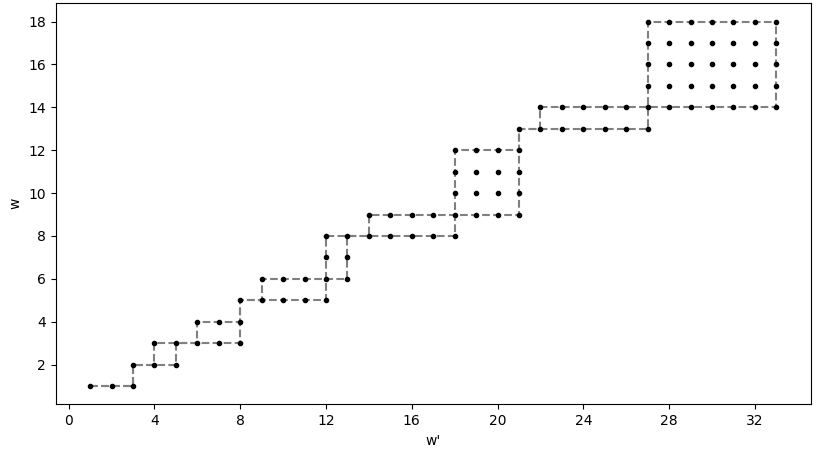
\includegraphics[scale=0.7]{w-n.png}

\vspace{1cm}
\begin{definition}[Joint function]
	Define the function $\eta : (\min\{s, t\}, \infty) \to \mathbb{Z}^+$
	\begin{align*}
		\eta(x) = \begin{cases} 1  &(\min\{s, t\}<x\le s+t)\\
			\eta(x-s) + \eta(x-t)  &(x> s+t)
		\end{cases}
	\end{align*}
	This function is like stair cases, and has the form
	\begin{align*}
		\eta(x) = \begin{cases} \eta_1  &(\min\{s, t\}<x\le x_1)\\
			\eta_2  &(x_1<x\le x_2)\\
			\eta_3  &(x_2<x\le x_3)\\
			\eta_4  &(x_3<x\le x_4)\\
			\cdots
		\end{cases}
	\end{align*}
	where $\eta_1 = 1$,  $x_1 = s+t$ and the function is non-decreasing. It defines the ``joint sequence" $\{\eta_k\}_{k=1}^{\infty}$ that's strictly increasing
	\[
	\eta_1 < \eta_2 < \eta_3 < \eta_4 < \dots
	\]
	
	We call a tuple $(x_k, \eta_k\nearrow\eta_{k+1})$ a ``jump point".
\end{definition}

\vspace{1cm}
\begin{lemma}[Joint]
	 Each jump point is related to $E(n)$ in the range $n \in [\eta_k, \eta_{k+1})$. For $\eta_k \le n < \eta_{k+1}$
	\begin{align*}
	\Delta E_{s,t}(n) &= x_k\\
	w^{\min}_{s,t}(n) &= \max\{\eta(x_k-t),\, \eta(x_{k+1}-t) + n -\eta_{k+1}\}\quad(n\geq 2)	\\
	w^{\max}_{s,t}(n) &= \min\{\eta(x_{k+1}-t),\,\eta(x_k-t) + n -\eta_k \} \quad(n\geq 2)
	\end{align*}
	Specifically
	\[
	w_{s,t}(\eta_k) = \{\eta(x_k-t)\}\quad(\eta_k\geq 2)
	\]
	In other words, a jump point corresponds to a bead $B(w_{\triangleleft}, w_{\triangleright}, n_{\triangleleft},n_{\triangleright})$ defined by
	\begin{align*}
	n_{\triangleleft} &= \eta_k\\
	n_{\triangleright} &= \eta_{k+1}\\
	w_{\triangleleft} &= \eta(x_k - t)\\
	w_{\triangleright} &= \eta(x_{k+1} - t)\\
	w'_{\triangleleft} &= \eta(x_k - s)\\
	w'_{\triangleright} &= \eta(x_{k+1} - s)
	\end{align*}
\end{lemma}
\begin{proof}
		Proof by induction
	\paragraph{Base case}
	The first jump point is $(x_1, \eta_1\nearrow\eta_2) = (s+t, 1\nearrow2)$, which corresponds to $n = 1$. We have shown that $\Delta E(1) = s + t$ so the base case is satisfied.

	\paragraph{Inductive step} A jump point $(x_k, \eta_k\nearrow\eta_{k+1})$, is related to two previous ``probable jump points" $(x_k-s, S\nearrow_?S')$ and $(x_k-t, T\nearrow_?T')$, with the following relation
	\begin{align*}
	S &= \eta(x_k-s)\\
	T &= \eta(x_k-t)\\
	S' &= \eta(x_{k+1}-s)\\
	T' &= \eta(x_{k+1}-t)\\
	S + T &= \eta_k \\
	S' + T' &= \eta_{k+1}
	\end{align*}
	At least one of the two probable jump points $x_k-s$, $x_k-t$ must be a real jump point (otherwise $x_k$ wouldn't be a jump point). And then we have the following inequalities
	\begin{align*}
	\Delta E(S) &\ge x_k - s &(\text{Equal when $x_k-s$ is a jump point}) \\
	\Delta E(T) &\ge x_k - t &(\text{Equal when $x_k-t$ is a jump point}) \\
	\Delta E(S+1) &\ge \Delta E(S) \ge x_k - s  &(\text{Due to convexity of $E$})\\
	\Delta E(T+1) &\ge \Delta E(T) \ge x_k - t \\
	\Delta E(S-1) &< x_k - s &(\text{if $S\ge 2$})\\
	\Delta E(T-1) &< x_k - t &(\text{if $T\ge 2$})\\
	\end{align*}
	Let's look at the starting point of the current interval $E(\eta_k)$ around $w = T$. The differential $\Delta_w D$ are
	\begin{align*}
	\Delta_w D^{T - 1}(\eta_k) &= \Delta E(T-1) - \Delta E(\eta_k - T) + t - s\\
	&= \Delta E(T-1) - \Delta E(S) + t - s\\
	&< (x_k - t) - (x_k - s) + t - s = 0
	\end{align*}
	\begin{align*}
	\Delta_w D^{T }(\eta_k) &= \Delta E(T) - \Delta E(\eta_k - T - 1) + t - s\\
	&= \Delta E(T) - \Delta E(S - 1) + t - s\\
	&> (x_k - t) - (x_k - s) + t - s = 0
	\end{align*}
	Either of them might not exist for $T = 1$ or $T = \eta_k - 1$, but it doesn't affect the arguments. Because of convexity of $D^w$, this means
	\[
	w(\eta_k) = \{T\} = \{\eta(x_k-t)\}
	\]
	and
	\[
	E(\eta_k) = E(T) + E(S) + T t + S s
	\]
	We can use the same argument for the last point of the current interval and get
	\[
	w(\eta_{k+1}) = \{T'\}
	\]
	\[
	E(\eta_{k+1}) = E(T') + E(S') + T' t + S' s
	\]
	The total difference between the two end points is
	\begin{align*}
	E(\eta_{k+1}) - E(\eta_k) &= E(T') - E(T) + E(S') - E(S) + (T'-T)t + (S'-S)s\\
	&= (T'-T)(x_k-t) + (S'-S)(x_k-s) + (T'-T)t + (S'-S)s \quad \\
	&(\text{This is true regardless whether the $x_k-t$ or $x_k-s$ is real jump points})\\
	&=(T'-T + S' - S)x_k\\
	&=(\eta_{k+1} -\eta_k)x_k
	\end{align*}
	If $\eta_{k+1} -\eta_k = 1$, then
	\[
	E(\eta_{k+1}) - E(\eta_k) = \Delta E(\eta_k) = x_k
	\]
	and the current interval is proved. Otherwise, let's look at $E(\eta_k +1)$ around $w = T$ and $w = T+1$. The differential $\Delta_w D$ are
	\begin{align*}
	\Delta_w D^{T - 1}(\eta_k+1) &= \Delta E(T-1) - \Delta E(\eta_k - T + 1) + t - s\\
	&=\Delta E(T-1) - \Delta E(S + 1) + t - s\\
	&< (x_k - t) - (x_k -s) + t -s = 0
	\end{align*}
	\begin{align*}
	\Delta_w D^{T + 1}(\eta_k+1) &= \Delta E(T+1) - \Delta E(\eta_k - T - 1) + t - s\\
	&=\Delta E(T+1) - \Delta E(S - 1) + t - s\\
	&> (x_k - t) - (x_k -s) + t -s = 0
	\end{align*}
	Again, either of them might not exist, but anyway, due to convexity, the optimizer is among $w\in\{T, T+1\}$ (or potentially both). Their $D^w(\eta_k+1)$ are
	\begin{align*}
	D^T(\eta_k+1) &= E(T) + E(\eta_k+1-T) +Tt +(\eta_k+1-T)s \\
	&= E(T) + E(S+1) +Tt +(S+1)s\\
	&= E(T) + E(S) + \Delta E(S) +Tt +(S+1)s\\
	&= E(\eta_k) + \Delta E(S) +s \\
	&\geq E(\eta_k) + x_k \quad (\text{equality holds when $x_k-s$ is a jump point})
	\end{align*}
	\begin{align*}
	D^{T+1}(\eta_k+1) &= E(T+1) + E(\eta_k-T) +(T+1)t +(\eta_k-T)s \\
	&= E(T+1) + E(S) +(T+1)t +Ss \\
	&= E(T) + \Delta E(T)+ E(S) +  (T+1)t +Ss\\
	&= E(\eta_k) + \Delta E(T) +t \\
	&\geq E(\eta_k) + x_k \quad (\text{equality holds when $x_k-t$ is a jump point})
	\end{align*}
	Because at least one of the equality holds, we have
	\[
	E(\eta_k+1) =  E(\eta_k) + x_k
	\]
	The choice of $w$ among $\{T, T+1\}$ depends on which are jump points
	\begin{itemize}
		\item $x_k-s$ is a jump point $\iff T \in w(\eta_k+1)$
		\item $x_k-t$ is a jump point $\iff T+1 \in w(\eta_k+1)$
	\end{itemize}
	Then $\Delta E(\eta_k)$ would be
	\begin{align*}
	\Delta E(\eta_k) &= E(\eta_k+1) - E(\eta_k) \\
	&= x_k
	\end{align*}
	Remember $E(\eta_{k+1}) - E(\eta_k) = (\eta_{k+1} -\eta_k)x_k$, then we have
	\begin{align*}
	(\eta_{k+1} -\eta_k)x_k &= E(\eta_{k+1}) - E(\eta_k) \\
	&= \Delta E(\eta_k) + \Delta E(\eta_k + 1) +\dots+\Delta E(\eta_{k+1} - 1) \\
	&\geq  \Delta E(\eta_k) + \Delta E(\eta_k) +\dots+\Delta E(\eta_k) \\
	&\geq (\eta_{k+1} -\eta_k)x_k
	\end{align*}
	This equality must holds, so this locks all $\Delta E(n) = x_k$ for $\eta_{k} \leq n < \eta_{k+1}$, and this proves the formula for $\Delta E(n)$.

	As for the values of $w(n)$ in between, we have three cases
	\begin{itemize}
		\item If both $x_k-s$ and $x_k-t$ are jump points, then we have $w(\eta_k +1) =\{T, T+1\}$, and $E(n)$ is linear for $n \in [S, S']$ and $n \in [T, T']$. We have shown that $w(n)$ will form a parallelogram that satisfy the formula.
		\item If $x_k-s$ is not a jump point, then we have the following equations
		\begin{align*}
		S &= S'\\
		w(\eta_{k}) &= \{T\}\\
		w(\eta_{k+1}) &= \{T'\} = \{T+\eta_{k+1} - \eta_k\}
		\end{align*}
		The two end points form a slope of 1. Because of $w$-Lipschitz continuity, this forces all $w(n)$ to be on the thin line $w(\eta_{k} + a) = \{T+a\}$.
		\item If $x_k-t$ is not a jump point, then we have the following equations
		\begin{align*}
		T &= T'\\
		w(\eta_{k}) &= \{T\}\\
		w(\eta_{k+1}) &= \{T'\} = \{T\}
		\end{align*}
		The two end points are on the same level. Because of $w$-Lipschitz continuity, this forces all $w(n)$ to be on the same level.
	\end{itemize}
	In summary, we have proved the formula for $w(n)$


\end{proof}

\paragraph{Remark}

Although we defined $\eta(n)$ on all real numbers in $(\min\{s, t\}, \infty)$, not all of them are important. It is easy to see that jump points $x_k$ can only be in the following subsets
\begin{itemize}
	\item for $s/t\in\mathbb{Q}$, $x_k \in \gcd(s,t)\mathbb{Z}$. Specifically, if $s$ and $t$ are integers, all  $x_k$ is a subset of $\mathbb{Z}$. We will discuss this in the next section.
	\item for $s/t\notin\mathbb{Q}$, $x_k \in s\mathbb{Z} + t\mathbb{Z}$, a subset of an algebraic number field with bases $\{s, t\}$
\end{itemize}
Another way to put this is that the jump point sequence $\{x_k\}_{k=1}^{\infty}$ is all elements in ascending order from the set
\[
	J_{s,t} = \{ps+qt\ |\  p \in \mathbb{Z}^+, q \in \mathbb{Z}^+\}
\]

The function $\Delta E(n)$ is, in some sense, the inverse function of $\eta(x)$. Of course, $\eta(x)$ is not injective, so we take the inverse in this way: for each flat line in $\eta(n)$ which becomes vertical in the inverse, we take the highest point as the inverse function value. We also connects the vertical jumps in $\eta(n)$, which becomes flat in the inverse. The $\Delta E(n)$ function, defined over $n \in [1, \infty)$ (for real numbers) is
\begin{align*}
\Delta E(n) = \begin{cases}
x_1 & (1 = \eta_1 \le n < \eta_2) \\
x_2 & (\eta_2 \le n < \eta_3) \\
x_3 & (\eta_3 \le n < \eta_4) \\
\dots
\end{cases}
\end{align*}
and the function $E(n)$ is the integral
\begin{align*}
E(n) &= \int_1^n \Delta E(m)\, dm \\
 &= \left(\sum_{k = 1}^{h-1} x_k (\eta_{k+1} - \eta_k)\right) + x_{h} (n - \eta_{h}) \quad (\eta_{h} \le n < \eta_{h+1}) \\
 &= n x_h - \left(\eta_1 \min\{s, t\} + \int_{\min\{s, t\}}^{x_h} \eta(x)\, dx\right)\\
 &= n x_h  - \left(\eta_1 x_1 + \sum_{k=2}^{h} \eta_k (x_{h} - x_{h-1})\right)
\end{align*}
This also conforms to a natural extension of $E(n)$ for real number $n$: it is linear interpolation between nearest integer points.

Below is the graph of $n = \eta(x)$ and $x = \Delta E(n)$ for $s = \sqrt{2}, t = \sqrt{3}$.

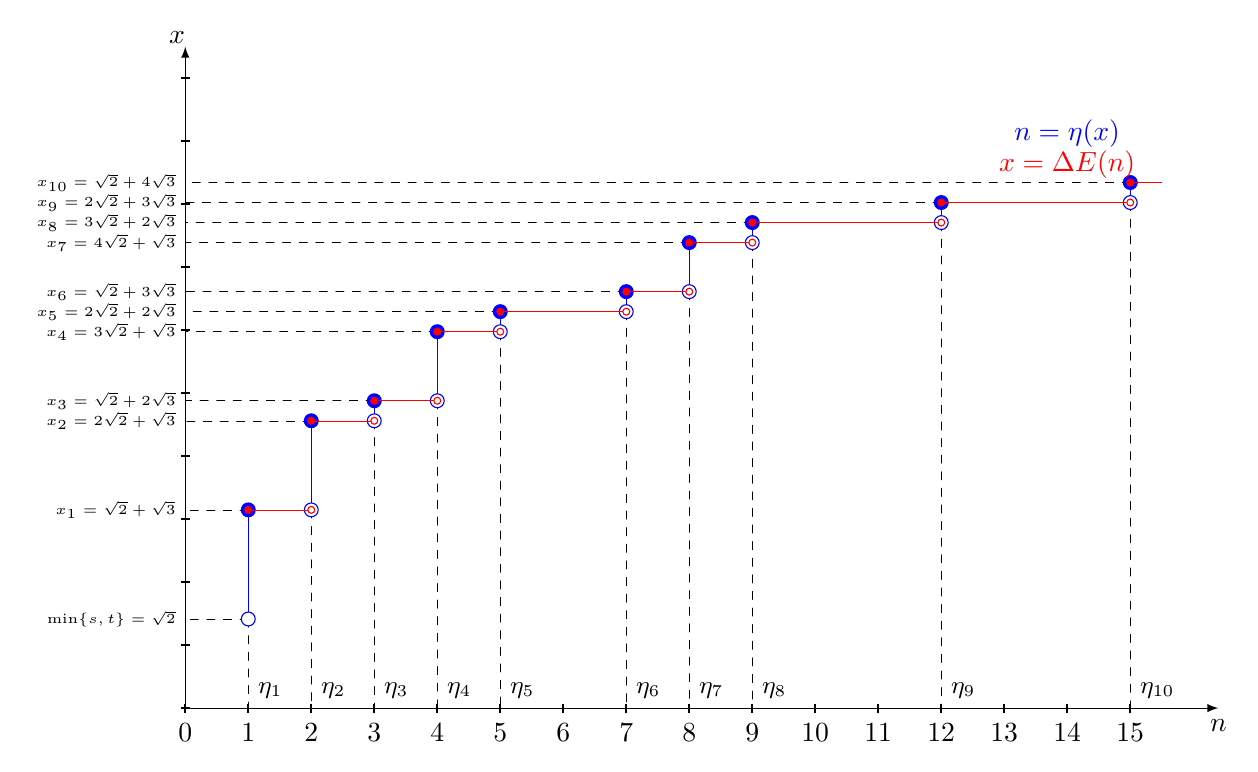
\begin{tikzpicture}[yscale=0.8,xscale=0.8]
\tkzInit[xmin=0,ymin=0,xmax=15.9,ymax=10,xstep=1,ystep=1]
\tkzDrawX[label={$n$}]
\tkzLabelX[step=1]
\tkzDrawY[label={$x$},above]
%\tkzLabelY[step=1]
\tkzDefPoint( 1, 3.1462643699419726){p0}
\tkzDefPoint( 2, 4.5604779323150675){p1}
\tkzDefPoint( 3, 4.878315177510849 ){p2}
\tkzDefPoint( 4, 5.974691494688162 ){p3}
\tkzDefPoint( 5, 6.292528739883945 ){p4}
\tkzDefPoint( 7, 6.610365985079727 ){p5}
\tkzDefPoint( 8, 7.388905057061258 ){p6}
\tkzDefPoint( 9, 7.70674230225704  ){p7}
\tkzDefPoint(12, 8.024579547452822 ){p8}
\tkzDefPoint(15, 8.342416792648605 ){p9}

\tkzDefPoint(0, 1.4142135623730950){pp}
\tkzDefPoint(0, 3.1462643699419726){pp0}
\tkzDefPoint(0, 4.5604779323150675){pp1}
\tkzDefPoint(0, 4.878315177510849 ){pp2}
\tkzDefPoint(0, 5.974691494688162 ){pp3}
\tkzDefPoint(0, 6.292528739883945 ){pp4}
\tkzDefPoint(0, 6.610365985079727 ){pp5}
\tkzDefPoint(0, 7.388905057061258 ){pp6}
\tkzDefPoint(0, 7.70674230225704  ){pp7}
\tkzDefPoint(0, 8.024579547452822 ){pp8}
\tkzDefPoint(0, 8.342416792648605 ){pp9}

\tkzDefPoint( 1, 1.4142135623730950){q}
\tkzDefPoint( 2, 3.1462643699419726){q0}
\tkzDefPoint( 3, 4.5604779323150675){q1}
\tkzDefPoint( 4, 4.878315177510849 ){q2}
\tkzDefPoint( 5, 5.974691494688162 ){q3}
\tkzDefPoint( 7, 6.292528739883945 ){q4}
\tkzDefPoint( 8, 6.610365985079727 ){q5}
\tkzDefPoint( 9, 7.388905057061258 ){q6}
\tkzDefPoint(12, 7.70674230225704  ){q7}
\tkzDefPoint(15, 8.024579547452822 ){q8}
\tkzDefPoint(15.5, 8.342416792648605 ){qe}

\tkzDefPoint( 1, 0){qq}
\tkzDefPoint( 2, 0){qq0}
\tkzDefPoint( 3, 0){qq1}
\tkzDefPoint( 4, 0){qq2}
\tkzDefPoint( 5, 0){qq3}
\tkzDefPoint( 7, 0){qq4}
\tkzDefPoint( 8, 0){qq5}
\tkzDefPoint( 9, 0){qq6}
\tkzDefPoint(12, 0){qq7}
\tkzDefPoint(15, 0){qq8}

\tkzDrawSegments[style=dashed](q,pp p0,pp0 p1,pp1 p2,pp2 p3,pp3 p4,pp4 p5,pp5 p6,pp6 p7,pp7 p8,pp8 p9,pp9)
\tkzDrawSegments[style=dashed](q,qq q0,qq0 q1,qq1 q2,qq2 q3,qq3 q4,qq4 q5,qq5 q6,qq6 q7,qq7 q8,qq8)

\tkzDrawSegments[color=blue](q,p0 q0,p1 q1,p2 q2,p3 q3,p4 q4,p5 q5,p6 q6,p7 q7,p8 q8,p9)
\tkzDrawPoints[size=5,color=blue](p0,p1,p2,p3,p4,p5,p6,p7,p8,p9)
\tkzDrawPoints[size=5,color=blue,fill=white](q,q0,q1,q2,q3,q4,q5,q6,q7,q8)

\tkzDrawSegments[color=red](p0,q0 p1,q1 p2,q2 p3,q3 p4,q4 p5,q5 p6,q6 p7,q7 p8,q8 p9,qe)
\tkzDrawPoints[size=2.5,color=red](p0,p1,p2,p3,p4,p5,p6,p7,p8,p9)
\tkzDrawPoints[size=2.5,color=red,fill=white](q0,q1,q2,q3,q4,q5,q6,q7,q8)


\tkzLabelPoint[color=blue]({14,9.5}){$n = \eta(x)$}
\tkzLabelPoint[color=red]({14,9}){$x = \Delta E(n)$}

\tkzLabelPoint[left](pp){\tiny $\min\{s,t\}=\sqrt{2}$}
\tkzLabelPoint[left](pp0){\tiny $x_1=\sqrt{2}+\sqrt{3}$}
\tkzLabelPoint[left](pp1){\tiny $x_2=2\sqrt{2}+\sqrt{3}$}
\tkzLabelPoint[left](pp2){\tiny $x_3=\sqrt{2}+2\sqrt{3}$}
\tkzLabelPoint[left](pp3){\tiny $x_4=3\sqrt{2}+\sqrt{3}$}
\tkzLabelPoint[left](pp4){\tiny $x_5=2\sqrt{2}+2\sqrt{3}$}
\tkzLabelPoint[left](pp5){\tiny $x_6=\sqrt{2}+3\sqrt{3}$}
\tkzLabelPoint[left](pp6){\tiny $x_7=4\sqrt{2}+\sqrt{3}$}
\tkzLabelPoint[left](pp7){\tiny $x_8=3\sqrt{2}+2\sqrt{3}$}
\tkzLabelPoint[left](pp8){\tiny $x_9=2\sqrt{2}+3\sqrt{3}$}
\tkzLabelPoint[left](pp9){\tiny $x_{10}=\sqrt{2}+4\sqrt{3}$}

\tkzLabelPoint[above right](qq){\small $\eta_1$}
\tkzLabelPoint[above right](qq0){\small $\eta_2$}
\tkzLabelPoint[above right](qq1){\small $\eta_3$}
\tkzLabelPoint[above right](qq2){\small $\eta_4$}
\tkzLabelPoint[above right](qq3){\small $\eta_5$}
\tkzLabelPoint[above right](qq4){\small $\eta_6$}
\tkzLabelPoint[above right](qq5){\small $\eta_7$}
\tkzLabelPoint[above right](qq6){\small $\eta_8$}
\tkzLabelPoint[above right](qq7){\small $\eta_9$}
\tkzLabelPoint[above right](qq8){\small $\eta_{10}$}

\end{tikzpicture}



\vspace{1cm}
\begin{definition}[Jump height function] Define $\delta: (\min\{s,t\},\infty)\to\mathbb{Z}^{0+}$
	\[
	\delta(x) = \eta(x^+) - \eta(x^-) =\begin{cases}
		\eta_{i+1} - \eta_{i} & (x = x_i)\\
		0 & (\text{otherwise})\\
	\end{cases}
	\]
	which can also be expressed with the recursive formula
	\begin{align*}
		\delta(x) = \begin{cases}
			0 & (x \in (\min\{s, t\}, s + t))\\
			1 & (x = s+t)\\
			\delta(x-s)+ \delta(x-t) & (x\in(s+t,\infty))
		\end{cases}
	\end{align*}
	
\end{definition}

\vspace{1cm}
\begin{lemma}[Jump height formula]
	\[
	\delta(x) = \sum_{(p,q)\in(\mathbb{Z}^+)^2}^{ps+qt = x} \frac{(p+q-2)!}{(p-1)!(q-1)!}
	\]
\end{lemma}
\begin{proof}
	For $s/t\notin\mathbb{Q}$, the jump point set $J_{s,t}$ has one-to-one correspondence to positive integer pairs $(p,q)\in(\mathbb{Z}^+)^2$. This means, for $(p,q)\in(\mathbb{Z}^{0+})^2 / \{(0,0), (0,1), (1,0)\}$
	\begin{align*}
		\delta(ps+qt) = \begin{cases}
			0 & (p= 0 \text{ or } q = 0) \\
			1 & (p = q = 1) \\
			\delta((p-1)s+qt) + \delta(ps+(q-1)t) & (\text{otherwise})
		\end{cases}
	\end{align*}
	It is easy to see $\delta$ forms a Pascal's triangle over $(p,q)\in(\mathbb{Z}^+)^2$
	\[
	\delta(ps+qt) = \binom{p+q-2}{q-1} = \frac{(p+q-2)!}{(p-1)!(q-1)!}
	\]
	This can be further generalized to make it also work for $s/t\in\mathbb{Q}$ as
	\[
	\delta(x) = \sum_{(p,q)\in(\mathbb{Z}^+)^2}^{ps+qt = x} \frac{(p+q-2)!}{(p-1)!(q-1)!}
	\]
	To see how this works for rational $s/t$, we can still map $x$ to integer pair $(p, q)$ - except this time a line of many $(p, q)$ correspond to the same $x$. For the first jump point $x = s + t$, all $(p, q)$ such that $ps + qt = s + t$ will have corresponding $\delta = 1$. This is equivalent to ``seeding" Pascal's triangles at many places, so the resulting $\delta$ value everywhere should be the sum of all these Pascal's triangles.
	
\end{proof}


\vspace{1cm}
\begin{lemma}[Pascal joints]
	\[
	\eta(x) = 1 + \sum_{x_i < x} \delta(x_i) = 1 + \sum_{(p,q)\in(\mathbb{Z}^+)^2}^{ps+qt < x} \frac{(p+q-2)!}{(p-1)!(q-1)!}
	\]
\end{lemma}

\vspace{1cm}
\begin{definition}[Midpoint joins]
	Define the slightly modified function $\eta_0(x)$ as 
	\[
	\eta_0(x) = \lim_{\varepsilon\to 0} \frac{1}{2}(\eta(x-\varepsilon) + \eta(x+\varepsilon))
	\]
\end{definition}

\vspace{1cm}
\begin{lemma}[Laplace joints]
	\[
	\eta_0(x) =  \sum_r \frac{e^{rx}}{r(s e^{tr} + t e^{sr})}
	\]
	where $r$ are all complex roots of equation
	\[
	e^{-sr} + e^{-tr} = 1
	\]
\end{lemma}

\begin{proof}

Consider the following shifted function $\phi(x)$
\begin{align*}
	\phi(x) &= \eta_0(x + s +t) \\
	&= 1 + \sum_{(p,q)\in(\mathbb{Z}^+)^2}^{ps+qt < x+s+t} \frac{(p+q-2)!}{(p-1)!(q-1)!}\\
	&= 1 + \sum_{(p,q)\in(\mathbb{Z}^{0+})^2}^{ps+qt < x} \frac{(p+q)!}{p!q!}\\
	&= 1 + \sum_{p=0}^{\infty}\sum_{q=0}^{\infty} \frac{(p+q)!}{p!q!} \theta(x - (ps + qt))
\end{align*}
where $\theta$ is the unit step function. Its Laplace transform is
\begin{align*}
\mathcal{L}\{\phi\}(\sigma) &= \frac{1}{\sigma} + \sum_{p=0}^{\infty}\sum_{q=0}^{\infty} \frac{(p+q)!}{p!q!} \frac{e^{-(ps+qt)\sigma}}{\sigma} \\
&= \frac{1}{\sigma} + \frac{1}{\sigma} \sum_{j=0}^{\infty} (e^{-s\sigma} + e^{-t\sigma})^j\\
&= \frac{1}{\sigma} + \frac{1}{\sigma(1- (e^{-s\sigma} + e^{-t\sigma}))} \quad(\text{converges for big enough }\mathfrak{R}(\sigma))
\end{align*}
This function, after analytic continuation, has a removable singularity at $\sigma = 0$, and a pole at every $\sigma = r$ where $r$ are the complex roots of the following equation
\begin{align*}
e^{-sr} + e^{-tr} = 1
\end{align*}
On the other hand, function $\phi$ satisfy the functional equation
\[
\phi(x) = \phi(x - s) + \phi(x - t)
\]
which has a solution space with basis
\[
\phi_r(x) = e^{r x}
\]
where $r$ is a root of the same equation above. Function $\phi$ should be a linear combination of basis
\[
\phi(x) = \sum_{r} C_r e^{r x}
\]
which has Laplace transform that also has poles at $\sigma = r$
\[
\mathcal{L}\{\phi\}(\sigma) = \sum_{r} \frac{C_r}{\sigma - r}
\]
The two Laplace transform should agree to each other, so we can compare their coefficient of $1/(\sigma - r)$ at poles
\begin{align*}
C_r &= \lim_{\sigma\to r} \frac{\sigma - r}{\sigma(1- (e^{-s\sigma} + e^{-t\sigma}))} \\
&= \lim_{\sigma\to r} \frac{\partial_\sigma(\sigma - r)}{\sigma\partial_\sigma(1- (e^{-s\sigma} + e^{-t\sigma}))} \\
    &= \frac{1}{r(s e^{-sr} + t e^{-tr})}
\end{align*}
Plugging everything back, we get the new formula for $\eta_0(x)$
\[
\eta_0(x) = \sum_r \frac{e^{r(x - (s +t))}}{r(s e^{-sr} + t e^{-tr})}  = \sum_r \frac{e^{rx}}{r(s e^{tr} + t e^{sr})}
\]
Note that this series doesn't converge absolutely and summation order is important. We can index $r$ by $|\mathfrak{I}(r)|$ in ascending order. This follows the limit direction in Mellin's inverse formula, together with Cauchy residue theorem.

\end{proof}

\vspace{1cm}
\begin{definition}[Pascal]
	Define the following tuple sets
	\[
	\Omega^E_{s,t} = \left\{\left(\binom{p+q-2}{p-1}, ps+qt \right) \ \middle|\ (p,q)\in(\mathbb{Z}^+)^2 \right\}
	\]
	\[
	\Omega^w_{s,t} = \left\{\left(\binom{p+q-3}{q-2}, \binom{p+q-3}{p-2}, ps+qt \right) \ \middle|\ (p,q)\in(\mathbb{Z}^+)^2 \backslash (1,1) \right\}
	\]
\end{definition}

\vspace{1cm}
\begin{lemma}[Pascal]
	$E(n)$ and $w(n)$ can be generated from $\Omega^E_{s,t}$ and $\Omega^w_{s,t}$
\end{lemma}
\begin{proof}

Sort all elements in $\Omega^E_{s,t}$ by $ps+qt$ in ascending order. For equal elements, the order doesn't matter. Then starting from $n=1$, each element generates a segment in $E(n)$ with the length of $\binom{p+q-2}{p-1}$, and slope ($\Delta n$) of $(ps+qt)$.


Sort all elements in $\Omega^w_{s,t}$ by $ps+qt$ in ascending order. This time for equal elements, we combine them into one element by calculating the sum of $\binom{p+q-3}{q-2}$ and $\binom{p+q-3}{p-2}$. We then connect all vectors $\left(\binom{p+q-3}{q-2}, \binom{p+q-3}{p-2}\right)$ head to tail, starting from $(1,1)$. Each vector becomes a segment $(w_{\triangleleft}, w'_{\triangleleft}) - (w_{\triangleright}, w'_{\triangleright})$, each corresponds to a bead where
\begin{align*}
	n_\triangleleft &= w_{\triangleleft} + w'_{\triangleleft} \\
	n_\triangleright &= w_{\triangleright} + w'_{\triangleright} \\
\end{align*}

\end{proof}

\vspace{1cm}
\begin{definition}[Middle]
	For each bead $	B(n_{\triangleleft}, n_{\triangleright}, w_{\triangleleft}, w_{\triangleright})$, define $w^{\ominus}_{s,t}(n)$ as the linear interpolation on real number between $[n_{\triangleleft}, n_{\triangleright}]$
	\[
		w^{\ominus}_{s,t}(n) = \frac{n - n_{\triangleleft}}{n_{\triangleright} - n_{\triangleleft}} w_{\triangleright} + \frac{n_{\triangleright} - n}{n_{\triangleright} - n_{\triangleleft}}w_{\triangleleft}
	\]
	Since beads are connected, this defines a function $w_{s,t}^{\ominus}: [2, \infty)\to\mathbb{R}$
\end{definition}

\paragraph{Remark}
It can be seen that we always have
\[
w^{\min}(n)\le w^{\ominus}(n)\le w^{\max}(n)
\]

Each bead in the $w(n)$ graph is rectangle in the $w$-$w'$, and $w^{\ominus}$ are the rising diagonals. The following is the $w$-$w'$ graph of $w^{\ominus}$ for $s=4$, $t=9$

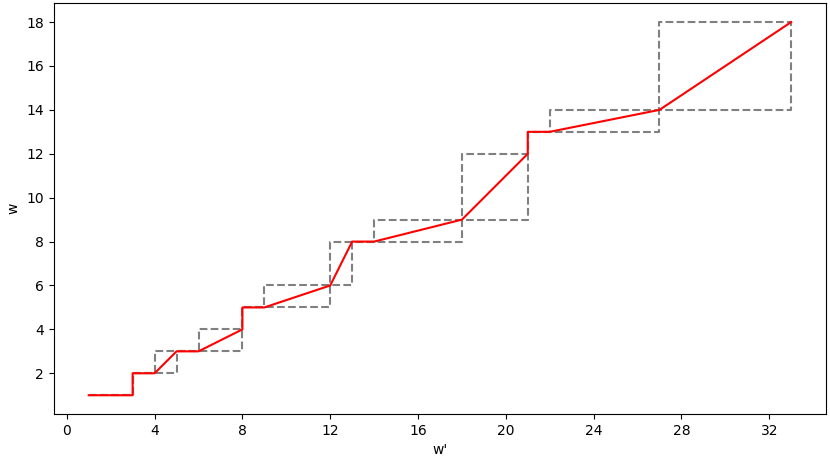
\includegraphics[scale=0.7]{w-n-v.png}

\vspace{1cm}
\begin{definition}[Fibonacci]
	Given positive integer $s$ and $t$, define the non-decreasing ``genfib sequence" (generalized Fibonacci sequence) $\{n_i\}_{i=\min\{s,t\}+1}^\infty$ as
	\[
	n_{\min\{s,t\}+1} = \dots = n_{s + t} = 1
	\]
	\[
	n_{i} = n_{i - s} + n_{i - t} , \quad i > s + t
	\]
\end{definition}

\vspace{1cm}
\begin{lemma}[Fibonacci]
	Given positive integer $s$ and $t$ and its genfib sequence, for $n_i \neq n_{i+1}$, for $n_i \le n < n_{i+1}$
	\begin{align*}
	\Delta E_{s,t}(n) &= i\\
	w^{\min}_{s,t}(n) &= \max\{n_{i - t},\, n_{i +1 - t} + n - n_{i+1}\}\quad(n\geq 2)	\\
	w^{\max}_{s,t}(n) &= \min\{n_{i +1 - t},\,n_{i - t} + n - n_{i} \} \quad(n\geq 2)
	\end{align*}
\end{lemma}
\begin{proof}
	We can construct $\{n_i\}_{i=\min\{s,t\}+1}^{\infty}$ from $\eta(x)$ as
	\[
	n_i = \eta(i)
	\]
	and one can easily verify that this satisfies the recurrence relation of both $\eta(x)$ and $\{n_i\}_{i}$. And for every $n_i \neq n_{i+1}$, there is a jump point at $(i,n_i\nearrow n_{i+1})$, and we can derive the $\Delta E_{s,t}(n)$ and $w_{s,t}(n)$ formula for integer case from the previous property.

\end{proof}

\paragraph{Remark}

This property provides a way to recursively generate linear segments for $E(n)$ when $s$ and $t$ are integers (and by extension due to homogeneity, whenever $s/t$ is rational). For example, for $s = t = 1$ (balanced bisection), we have the following
\begin{align*}
\Delta E_{1,1}(1) &= 2 \\
\Delta E_{1,1}(2) = \Delta E_{1,1}(3) &= 3\\
\Delta E_{1,1}(4) =\dots = \Delta E_{1,1}(7) &= 4\\
\Delta E_{1,1}(2^{i-2}) =\dots = \Delta E_{1,1}(2^{i-1}-1) &= i
\end{align*}
This forms a nice geometric progression.

Similarly, for $s = 1$ and $t = 2$, we have
\begin{align*}
\Delta E_{1,2}(1) &= 3 \\
\Delta E_{1,2}(2) &= 4\\
\Delta E_{1,2}(3)  = \Delta E_{1,2}(4) &= 5\\
\Delta E_{1,2}(5) =\dots = \Delta E_{1,2}(7) &= 6\\
\Delta E_{1,2}(8) =\dots = \Delta E_{1,2}(12) &= 7\\
\Delta E_{1,2}(\phi_{i -1}) =\dots = \Delta E_{1,2}(\phi_{i} - 1) &= i
\end{align*}
where $\phi_i$ is the $i$th Fibonacci number.

\vspace{1cm}
\begin{lemma}[Laplace Fibonacci]
	\[
	n_i = \sum_{\xi} \frac{\xi^{i}}{(\xi - 1)(s\xi^{t}+t\xi^{s})}
	\]
	where $\xi$ are the complex roots of equation
	\[
	\xi^{-s} + \xi^{-t} = 1
	\]
\end{lemma}
\begin{proof}
Similar to the continuous $\eta(x)$, we can also find an alternative formula for $n_i$. We first define
\[
\Phi_i = n_{i+s+t+1}
\]
then we can similarly derive
\[
\Phi_i = 1 + \sum_{p=0}^{\infty} \sum_{q=0}^{\infty}\frac{(p+q)!}{p!q!} \Theta(i-(ps+qt))
\]
where $\Theta$ is the integer unit step function $\Theta(i) = 1_{i \geq 0}$. This function has unilateral Z-transform
\begin{align*}
\mathcal{Z}\{\Phi\}(z) &= \frac{1}{1-z^{-1}}\left(1 +  \sum_{p=0}^{\infty} \sum_{q=0}^{\infty}\frac{(p+q)!}{p!q!} z^{-(ps+qt)} \right) \\
&= \frac{1}{1-z^{-1}}\left(1 +  \frac{1}{1-(z^{-s} + z^{-t})} \right)
\end{align*}
$\Phi_i$ should have an expansion in the form
\[
\Phi_i = \sum_{\xi} c_{\xi}\xi^i
\]
The expansion has Z-transform
\[
\mathcal{Z}\{\Phi\}(z) = \sum_{\xi} \frac{c_{\xi}}{1-\xi z^{-1}}
\]
Again by comparing coefficients at poles, we get
\[
c_{\xi} = \frac{1}{(1-\xi^{-1})(s\xi^{-s}+t\xi^{-t})}
\]
So we have
\[
n_i = \sum_{\xi} \frac{\xi^{i}}{(\xi - 1)(s\xi^{t}+t\xi^{s})}
\]
\end{proof}

\vspace{1cm}
\begin{lemma}[$s,t$-concavity]
Fixing $n$ and $s$, $E_{s,t}(n)$ as a function of $t$ is concave
\end{lemma}
\begin{proof}
Proof by induction. The base case $E_{s,t}(1) = 0$ is concave over $t$. In the recursive equation, all the summation components are concave, and the minimal of concave functions is still a concave function.
\end{proof}

\vspace{1cm}
\begin{lemma}[$s,t$-linearity]
Fixing $n$ and $s$, $E_{s,t}(n)$ is a piecewise linear function of $t$. The nodes are always at rational points.
\end{lemma}
\begin{proof}
	This can be proved by induction. Omitted.
\end{proof}

\paragraph{Remark}
With this property, we can graph the function with a series of segments. For example, the graph of $E_{1,t}(29)$ over $t\in[0,1]$ is

\vspace{0.5cm}
	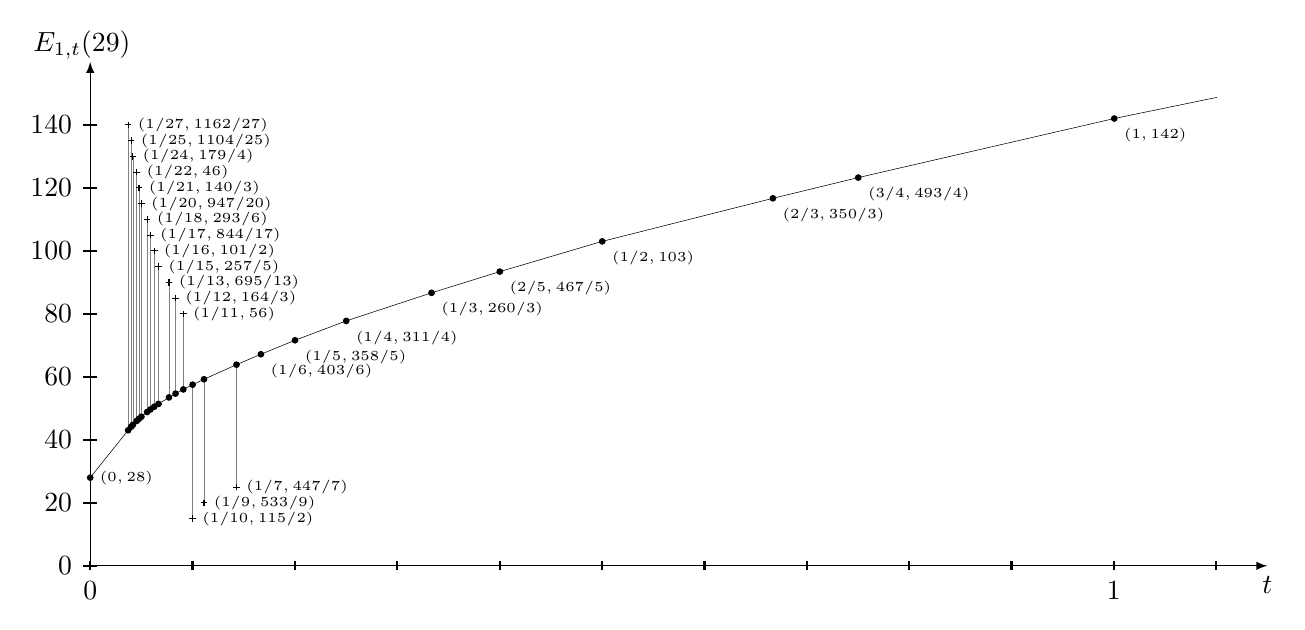
\begin{tikzpicture}[yscale=0.8,xscale=1.3]
	\tkzInit[xmin=0,ymin=0,xmax=1.1,ymax=150,xstep=0.1,ystep=20]
	\tkzDrawX[label={$t$}]
	\tkzLabelX[step=1]
	\tkzDrawY[label={$E_{1,t}(29)$},above]
	\tkzLabelY[step=10]

\tkzDefPoint(0,28){p0}
\tkzDefPoint(1/27,1162/27){p1} \tkzDrawSegment(p0,p1)
\tkzDefPoint(1/25,1104/25){p2} \tkzDrawSegment(p1,p2)
\tkzDefPoint(1/24,179/4){p3} \tkzDrawSegment(p2,p3)
\tkzDefPoint(1/22,46){p4} \tkzDrawSegment(p3,p4)
\tkzDefPoint(1/21,140/3){p5} \tkzDrawSegment(p4,p5)
\tkzDefPoint(1/20,947/20){p6} \tkzDrawSegment(p5,p6)
\tkzDefPoint(1/18,293/6){p7} \tkzDrawSegment(p6,p7)
\tkzDefPoint(1/17,844/17){p8} \tkzDrawSegment(p7,p8)
\tkzDefPoint(1/16,101/2){p9} \tkzDrawSegment(p8,p9)
\tkzDefPoint(1/15,257/5){p10} \tkzDrawSegment(p9,p10)
\tkzDefPoint(1/13,695/13){p11} \tkzDrawSegment(p10,p11)
\tkzDefPoint(1/12,164/3){p12} \tkzDrawSegment(p11,p12)
\tkzDefPoint(1/11,56){p13} \tkzDrawSegment(p12,p13)
\tkzDefPoint(1/10,115/2){p14} \tkzDrawSegment(p13,p14)
\tkzDefPoint(1/9,533/9){p15} \tkzDrawSegment(p14,p15)
\tkzDefPoint(1/7,447/7){p16} \tkzDrawSegment(p15,p16)
\tkzDefPoint(1/6,403/6){p17} \tkzDrawSegment(p16,p17)
\tkzDefPoint(1/5,358/5){p18} \tkzDrawSegment(p17,p18)
\tkzDefPoint(1/4,311/4){p19} \tkzDrawSegment(p18,p19)
\tkzDefPoint(1/3,260/3){p20} \tkzDrawSegment(p19,p20)
\tkzDefPoint(2/5,467/5){p21} \tkzDrawSegment(p20,p21)
\tkzDefPoint(1/2,103){p22} \tkzDrawSegment(p21,p22)
\tkzDefPoint(2/3,350/3){p23} \tkzDrawSegment(p22,p23)
\tkzDefPoint(3/4,493/4){p24} \tkzDrawSegment(p23,p24)
\tkzDefPoint(1,142){p25} \tkzDrawSegment(p24,p25)
\tkzDefPoint(1.1,148.7){p26} \tkzDrawSegment(p25,p26)
\tkzLabelPoint[right](p0){\tiny $(0,28)$}
\tkzDefPoint(1/27,140){p1l}\tkzDrawSegment[color=gray](p1,p1l)\tkzDrawPoints[shape=cross](p1l)\tkzLabelPoint[right](p1l){\tiny $(1/27,1162/27)$}
\tkzDefPoint(1/25,135){p2l}\tkzDrawSegment[color=gray](p2,p2l)\tkzDrawPoints[shape=cross](p2l)\tkzLabelPoint[right](p2l){\tiny $(1/25,1104/25)$}
\tkzDefPoint(1/24,130){p3l}\tkzDrawSegment[color=gray](p3,p3l)\tkzDrawPoints[shape=cross](p3l)\tkzLabelPoint[right](p3l){\tiny $(1/24,179/4)$}
\tkzDefPoint(1/22,125){p4l}\tkzDrawSegment[color=gray](p4,p4l)\tkzDrawPoints[shape=cross](p4l)\tkzLabelPoint[right](p4l){\tiny $(1/22,46)$}
\tkzDefPoint(1/21,120){p5l}\tkzDrawSegment[color=gray](p5,p5l)\tkzDrawPoints[shape=cross](p5l)\tkzLabelPoint[right](p5l){\tiny $(1/21,140/3)$}
\tkzDefPoint(1/20,115){p6l}\tkzDrawSegment[color=gray](p6,p6l)\tkzDrawPoints[shape=cross](p6l)\tkzLabelPoint[right](p6l){\tiny $(1/20,947/20)$}
\tkzDefPoint(1/18,110){p7l}\tkzDrawSegment[color=gray](p7,p7l)\tkzDrawPoints[shape=cross](p7l)\tkzLabelPoint[right](p7l){\tiny $(1/18,293/6)$}
\tkzDefPoint(1/17,105){p8l}\tkzDrawSegment[color=gray](p8,p8l)\tkzDrawPoints[shape=cross](p8l)\tkzLabelPoint[right](p8l){\tiny $(1/17,844/17)$}
\tkzDefPoint(1/16,100){p9l}\tkzDrawSegment[color=gray](p9,p9l)\tkzDrawPoints[shape=cross](p9l)\tkzLabelPoint[right](p9l){\tiny $(1/16,101/2)$}
\tkzDefPoint(1/15,95){p10l}\tkzDrawSegment[color=gray](p10,p10l)\tkzDrawPoints[shape=cross](p10l)\tkzLabelPoint[right](p10l){\tiny $(1/15,257/5)$}
\tkzDefPoint(1/13,90){p11l}\tkzDrawSegment[color=gray](p11,p11l)\tkzDrawPoints[shape=cross](p11l)\tkzLabelPoint[right](p11l){\tiny $(1/13,695/13)$}
\tkzDefPoint(1/12,85){p12l}\tkzDrawSegment[color=gray](p12,p12l)\tkzDrawPoints[shape=cross](p12l)\tkzLabelPoint[right](p12l){\tiny $(1/12,164/3)$}
\tkzDefPoint(1/11,80){p13l}\tkzDrawSegment[color=gray](p13,p13l)\tkzDrawPoints[shape=cross](p13l)\tkzLabelPoint[right](p13l){\tiny $(1/11,56)$}
\tkzDefPoint(1/10,15){p14l}\tkzDrawSegment[color=gray](p14,p14l)\tkzDrawPoints[shape=cross](p14l)\tkzLabelPoint[right](p14l){\tiny $(1/10,115/2)$}
\tkzDefPoint(1/9,20){p15l}\tkzDrawSegment[color=gray](p15,p15l)\tkzDrawPoints[shape=cross](p15l)\tkzLabelPoint[right](p15l){\tiny $(1/9,533/9)$}
\tkzDefPoint(1/7,25){p16l}\tkzDrawSegment[color=gray](p16,p16l)\tkzDrawPoints[shape=cross](p16l)\tkzLabelPoint[right](p16l){\tiny $(1/7,447/7)$}
\tkzLabelPoint[right,anchor=north west](p17){\tiny $(1/6,403/6)$}
\tkzLabelPoint[right,anchor=north west](p18){\tiny $(1/5,358/5)$}
\tkzLabelPoint[right,anchor=north west](p19){\tiny $(1/4,311/4)$}
\tkzLabelPoint[right,anchor=north west](p20){\tiny $(1/3,260/3)$}
\tkzLabelPoint[right,anchor=north west](p21){\tiny $(2/5,467/5)$}
\tkzLabelPoint[right,anchor=north west](p22){\tiny $(1/2,103)$}
\tkzLabelPoint[right,anchor=north west](p23){\tiny $(2/3,350/3)$}
\tkzLabelPoint[right,anchor=north west](p24){\tiny $(3/4,493/4)$}
\tkzLabelPoint[right,anchor=north west](p25){\tiny $(1,142)$}
\tkzDrawPoints(p0,p1,p2,p3,p4,p5,p6,p7,p8,p9,p10,p11,p12,p13,p14,p15,p16,p17,p18,p19,p20,p21,p22,p23,p24,p25)

	\end{tikzpicture}

We omitted the graph beyond $t=1$, but remember that it can be derived by $E_{1,t}(n) = t\cdot E_{1,1/t}(n)$ due to symmetry and homogeneity.

It can be seen from the graph that nodes are mostly at unit fractions $t = 1/p$, but there are also a few nodes at non-unit fractions close to $t=1$.
\vspace{1cm}
\begin{lemma}[$w$ segment]
	Fixing $n$ and $s$, $w_{s,t}(n)$ is a ``piecewise constant" function. Over a single segment of the piecewise function $E_{s,t}(n)$, the same set of $w$ is chosen. However, exactly at a node of piecewise function $E_{s,t}(n)$, $w_{s,t}(n)$ can take a unique value that is not an element of either the left segment or the right segment.
\end{lemma}
\begin{proof}
	Remember that $E_{s,t}(n)$ calculated by taking the $t$-pointwise minimum of a sequence of piecewise linear, convex functions $D^w(t)$ indexed by $w$. If the pointwise minimum results in a simple linear function over a $t$-interval, it must be resulted from the same set of $w$. This is because, if any $D^w_{s,t}(n)$ tries to join or leave $E_{s,t}(n)$ midway in the interval, it must bend down due to convexity, and that would result in  $E_{s,t}(n) \le D^w_{s,t}(n)$ bending down as well, contradicting with the fact that $E_{s,t}(n)$ is a simple linear function in this interval. $D^w_{s,t}(n)$ can only join or leave at the nodes of $E_{s,t}(n)$
\end{proof}

\paragraph{Remark}

If we graph $w$ over $t$, we will get a series of ``blocks", separated by vertical lines (marked red) at the nodes of $E$ over $t$. For example, the graph of $w_{1,t}(29)$ over $t\in[0,1]$ is (only the black part is the true value of $w$)

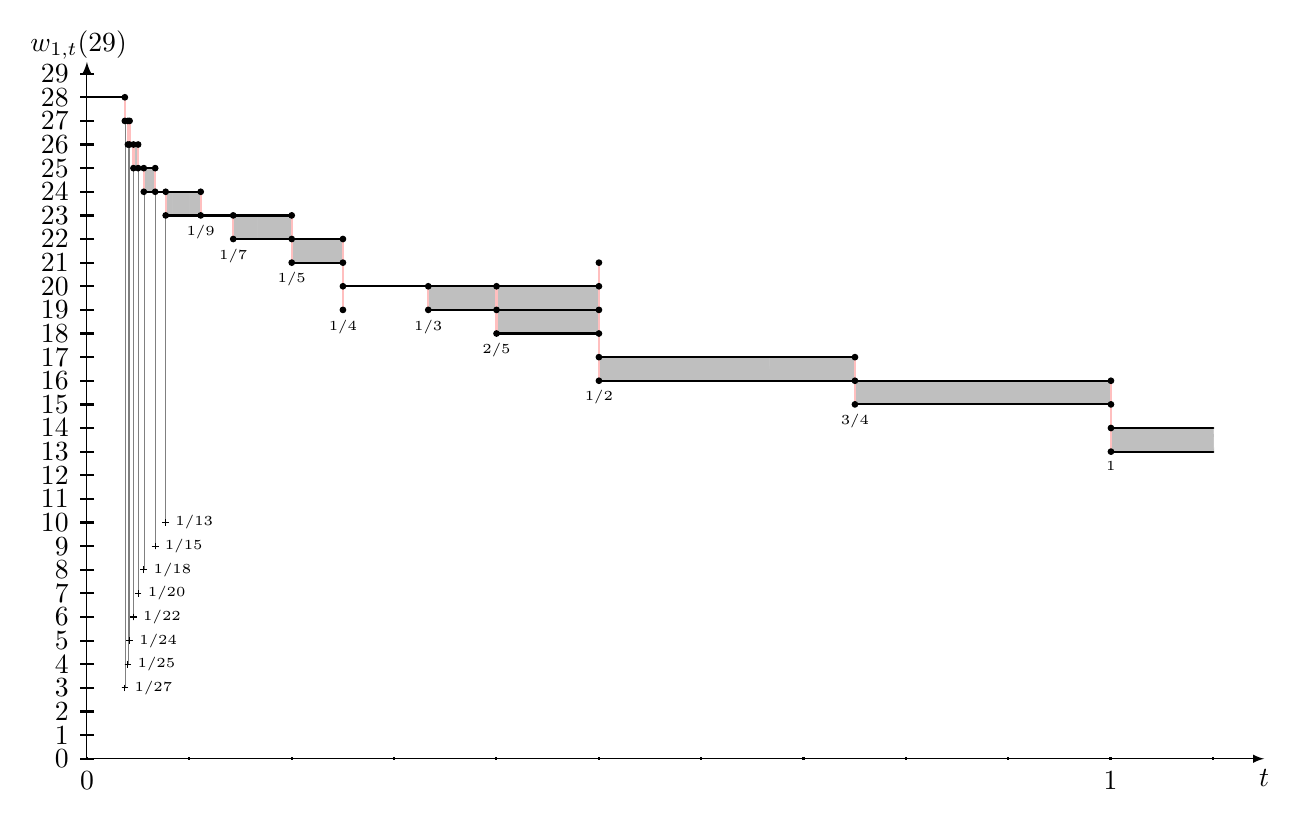
\begin{tikzpicture}[yscale=0.3,xscale=1.3]
\tkzInit[xmin=0,ymin=0,xmax=1.1,ymax=29,xstep=0.1,ystep=1]
\tkzDrawX[label={$t$}]
\tkzLabelX[step=1]
\tkzDrawY[label={$w_{1,t}(29)$},above]
\tkzLabelY[step=1]

\tkzDefPoint(    0,28){A}\tkzDefPoint( 1/27,28){C}\tkzDefRectangle(A,C)\tkzGetPoints{B}{D} \tkzDrawPolygon[fill=lightgray,draw=lightgray](A,...,D)
\tkzDefPoint( 1/27,27){A}\tkzDefPoint( 1/25,27){C}\tkzDefRectangle(A,C)\tkzGetPoints{B}{D} \tkzDrawPolygon[fill=lightgray,draw=lightgray](A,...,D)
\tkzDefPoint( 1/25,26){A}\tkzDefPoint( 1/24,27){C}\tkzDefRectangle(A,C)\tkzGetPoints{B}{D} \tkzDrawPolygon[fill=lightgray,draw=lightgray](A,...,D)
\tkzDefPoint( 1/24,26){A}\tkzDefPoint( 1/22,26){C}\tkzDefRectangle(A,C)\tkzGetPoints{B}{D} \tkzDrawPolygon[fill=lightgray,draw=lightgray](A,...,D)
\tkzDefPoint( 1/22,25){A}\tkzDefPoint( 1/21,26){C}\tkzDefRectangle(A,C)\tkzGetPoints{B}{D} \tkzDrawPolygon[fill=lightgray,draw=lightgray](A,...,D)
\tkzDefPoint( 1/21,25){A}\tkzDefPoint( 1/20,26){C}\tkzDefRectangle(A,C)\tkzGetPoints{B}{D} \tkzDrawPolygon[fill=lightgray,draw=lightgray](A,...,D)
\tkzDefPoint( 1/20,25){A}\tkzDefPoint( 1/18,25){C}\tkzDefRectangle(A,C)\tkzGetPoints{B}{D} \tkzDrawPolygon[fill=lightgray,draw=lightgray](A,...,D)
\tkzDefPoint( 1/18,24){A}\tkzDefPoint( 1/17,25){C}\tkzDefRectangle(A,C)\tkzGetPoints{B}{D} \tkzDrawPolygon[fill=lightgray,draw=lightgray](A,...,D)
\tkzDefPoint( 1/17,24){A}\tkzDefPoint( 1/16,25){C}\tkzDefRectangle(A,C)\tkzGetPoints{B}{D} \tkzDrawPolygon[fill=lightgray,draw=lightgray](A,...,D)
\tkzDefPoint( 1/16,24){A}\tkzDefPoint( 1/15,25){C}\tkzDefRectangle(A,C)\tkzGetPoints{B}{D} \tkzDrawPolygon[fill=lightgray,draw=lightgray](A,...,D)
\tkzDefPoint( 1/15,24){A}\tkzDefPoint( 1/13,24){C}\tkzDefRectangle(A,C)\tkzGetPoints{B}{D} \tkzDrawPolygon[fill=lightgray,draw=lightgray](A,...,D)
\tkzDefPoint( 1/13,23){A}\tkzDefPoint( 1/12,24){C}\tkzDefRectangle(A,C)\tkzGetPoints{B}{D} \tkzDrawPolygon[fill=lightgray,draw=lightgray](A,...,D)
\tkzDefPoint( 1/12,23){A}\tkzDefPoint( 1/11,24){C}\tkzDefRectangle(A,C)\tkzGetPoints{B}{D} \tkzDrawPolygon[fill=lightgray,draw=lightgray](A,...,D)
\tkzDefPoint( 1/11,23){A}\tkzDefPoint( 1/10,24){C}\tkzDefRectangle(A,C)\tkzGetPoints{B}{D} \tkzDrawPolygon[fill=lightgray,draw=lightgray](A,...,D)
\tkzDefPoint( 1/10,23){A}\tkzDefPoint(  1/9,24){C}\tkzDefRectangle(A,C)\tkzGetPoints{B}{D} \tkzDrawPolygon[fill=lightgray,draw=lightgray](A,...,D)
\tkzDefPoint(  1/9,23){A}\tkzDefPoint(  1/7,23){C}\tkzDefRectangle(A,C)\tkzGetPoints{B}{D} \tkzDrawPolygon[fill=lightgray,draw=lightgray](A,...,D)
\tkzDefPoint(  1/7,22){A}\tkzDefPoint(  1/6,23){C}\tkzDefRectangle(A,C)\tkzGetPoints{B}{D} \tkzDrawPolygon[fill=lightgray,draw=lightgray](A,...,D)
\tkzDefPoint(  1/6,22){A}\tkzDefPoint(  1/5,23){C}\tkzDefRectangle(A,C)\tkzGetPoints{B}{D} \tkzDrawPolygon[fill=lightgray,draw=lightgray](A,...,D)
\tkzDefPoint(  1/5,21){A}\tkzDefPoint(  1/4,22){C}\tkzDefRectangle(A,C)\tkzGetPoints{B}{D} \tkzDrawPolygon[fill=lightgray,draw=lightgray](A,...,D)
\tkzDefPoint(  1/4,20){A}\tkzDefPoint(  1/3,20){C}\tkzDefRectangle(A,C)\tkzGetPoints{B}{D} \tkzDrawPolygon[fill=lightgray,draw=lightgray](A,...,D)
\tkzDefPoint(  1/3,19){A}\tkzDefPoint(  2/5,20){C}\tkzDefRectangle(A,C)\tkzGetPoints{B}{D} \tkzDrawPolygon[fill=lightgray,draw=lightgray](A,...,D)
\tkzDefPoint(  2/5,18){A}\tkzDefPoint(  1/2,20){C}\tkzDefRectangle(A,C)\tkzGetPoints{B}{D} \tkzDrawPolygon[fill=lightgray,draw=lightgray](A,...,D)
\tkzDefPoint(  1/2,16){A}\tkzDefPoint(  2/3,17){C}\tkzDefRectangle(A,C)\tkzGetPoints{B}{D} \tkzDrawPolygon[fill=lightgray,draw=lightgray](A,...,D)
\tkzDefPoint(  2/3,16){A}\tkzDefPoint(  3/4,17){C}\tkzDefRectangle(A,C)\tkzGetPoints{B}{D} \tkzDrawPolygon[fill=lightgray,draw=lightgray](A,...,D)
\tkzDefPoint(  3/4,15){A}\tkzDefPoint(    1,16){C}\tkzDefRectangle(A,C)\tkzGetPoints{B}{D} \tkzDrawPolygon[fill=lightgray,draw=lightgray](A,...,D)
\tkzDefPoint(1,  13){A}\tkzDefPoint(1.1,14){C}\tkzDefRectangle(A,C)\tkzGetPoints{B}{D} \tkzDrawPolygon[fill=lightgray,draw=lightgray](A,...,D)
\tkzDefPoint(1/27,26+1){A}\tkzDefPoint(1/27,28){B}\tkzDrawSegment[color=pink,thick](A,B)\tkzDefPoint(1/27,3){C}\tkzDrawSegment[color=gray](A,C)\tkzDrawPoints[shape=cross](C)\tkzLabelPoint[right](C){\tiny 1/27}
\tkzDefPoint(1/25,25+1){A}\tkzDefPoint(1/25,27){B}\tkzDrawSegment[color=pink,thick](A,B)\tkzDefPoint(1/25,4){C}\tkzDrawSegment[color=gray](A,C)\tkzDrawPoints[shape=cross](C)\tkzLabelPoint[right](C){\tiny 1/25}
\tkzDefPoint(1/24,25+1){A}\tkzDefPoint(1/24,27){B}\tkzDrawSegment[color=pink,thick](A,B)\tkzDefPoint(1/24,5){C}\tkzDrawSegment[color=gray](A,C)\tkzDrawPoints[shape=cross](C)\tkzLabelPoint[right](C){\tiny 1/24}
\tkzDefPoint(1/22,24+1){A}\tkzDefPoint(1/22,26){B}\tkzDrawSegment[color=pink,thick](A,B)\tkzDefPoint(1/22,6){C}\tkzDrawSegment[color=gray](A,C)\tkzDrawPoints[shape=cross](C)\tkzLabelPoint[right](C){\tiny 1/22}
\tkzDefPoint(1/20,24+1){A}\tkzDefPoint(1/20,26){B}\tkzDrawSegment[color=pink,thick](A,B)\tkzDefPoint(1/20,7){C}\tkzDrawSegment[color=gray](A,C)\tkzDrawPoints[shape=cross](C)\tkzLabelPoint[right](C){\tiny 1/20}
\tkzDefPoint(1/18,23+1){A}\tkzDefPoint(1/18,25){B}\tkzDrawSegment[color=pink,thick](A,B)\tkzDefPoint(1/18,8){C}\tkzDrawSegment[color=gray](A,C)\tkzDrawPoints[shape=cross](C)\tkzLabelPoint[right](C){\tiny 1/18}
\tkzDefPoint(1/15,23+1){A}\tkzDefPoint(1/15,25){B}\tkzDrawSegment[color=pink,thick](A,B)\tkzDefPoint(1/15,9){C}\tkzDrawSegment[color=gray](A,C)\tkzDrawPoints[shape=cross](C)\tkzLabelPoint[right](C){\tiny 1/15}
\tkzDefPoint(1/13,22+1){A}\tkzDefPoint(1/13,24){B}\tkzDrawSegment[color=pink,thick](A,B)\tkzDefPoint(1/13,10){C}\tkzDrawSegment[color=gray](A,C)\tkzDrawPoints[shape=cross](C)\tkzLabelPoint[right](C){\tiny 1/13}
\tkzDefPoint(1/ 9,22+1){A}\tkzDefPoint(1/9, 24){B}\tkzDrawSegment[color=pink,thick](A,B)\tkzLabelPoint[below](A){\tiny 1/9}
\tkzDefPoint(1/ 7,21+1){A}\tkzDefPoint(1/7, 23){B}\tkzDrawSegment[color=pink,thick](A,B)\tkzLabelPoint[below](A){\tiny 1/7}
\tkzDefPoint(1/ 5,20+1){A}\tkzDefPoint(1/5, 23){B}\tkzDrawSegment[color=pink,thick](A,B)\tkzLabelPoint[below](A){\tiny 1/5}
\tkzDefPoint(1/ 4,18+1){A}\tkzDefPoint(1/4, 22){B}\tkzDrawSegment[color=pink,thick](A,B)\tkzLabelPoint[below](A){\tiny 1/4}
\tkzDefPoint(1/ 3,18+1){A}\tkzDefPoint(1/3, 20){B}\tkzDrawSegment[color=pink,thick](A,B)\tkzLabelPoint[below](A){\tiny 1/3}
\tkzDefPoint(2/ 5,17+1){A}\tkzDefPoint(2/5, 20){B}\tkzDrawSegment[color=pink,thick](A,B)\tkzLabelPoint[below](A){\tiny 2/5}
\tkzDefPoint(1/ 2,15+1){A}\tkzDefPoint(1/2, 21){B}\tkzDrawSegment[color=pink,thick](A,B)\tkzLabelPoint[below](A){\tiny 1/2}
\tkzDefPoint(3/ 4,14+1){A}\tkzDefPoint(3/4, 17){B}\tkzDrawSegment[color=pink,thick](A,B)\tkzLabelPoint[below](A){\tiny 3/4}
\tkzDefPoint(1,   12+1){A}\tkzDefPoint(1,   16){B}\tkzDrawSegment[color=pink,thick](A,B)\tkzLabelPoint[below](A){\tiny 1}
\tkzDefPoint(    0,28){X}\tkzDefPoint( 1/27,28){Y}\tkzDrawSegment[color=black,thick](X,Y)
\tkzDefPoint( 1/27,27){X}\tkzDefPoint( 1/25,27){Y}\tkzDrawSegment[color=black,thick](X,Y)
\tkzDefPoint( 1/25,26){X}\tkzDefPoint( 1/24,26){Y}\tkzDrawSegment[color=black,thick](X,Y)
\tkzDefPoint( 1/25,27){X}\tkzDefPoint( 1/24,27){Y}\tkzDrawSegment[color=black,thick](X,Y)
\tkzDefPoint( 1/24,26){X}\tkzDefPoint( 1/22,26){Y}\tkzDrawSegment[color=black,thick](X,Y)
\tkzDefPoint( 1/22,25){X}\tkzDefPoint( 1/21,25){Y}\tkzDrawSegment[color=black,thick](X,Y)
\tkzDefPoint( 1/22,26){X}\tkzDefPoint( 1/21,26){Y}\tkzDrawSegment[color=black,thick](X,Y)
\tkzDefPoint( 1/21,25){X}\tkzDefPoint( 1/20,25){Y}\tkzDrawSegment[color=black,thick](X,Y)
\tkzDefPoint( 1/21,26){X}\tkzDefPoint( 1/20,26){Y}\tkzDrawSegment[color=black,thick](X,Y)
\tkzDefPoint( 1/20,25){X}\tkzDefPoint( 1/18,25){Y}\tkzDrawSegment[color=black,thick](X,Y)
\tkzDefPoint( 1/18,24){X}\tkzDefPoint( 1/17,24){Y}\tkzDrawSegment[color=black,thick](X,Y)
\tkzDefPoint( 1/18,25){X}\tkzDefPoint( 1/17,25){Y}\tkzDrawSegment[color=black,thick](X,Y)
\tkzDefPoint( 1/17,24){X}\tkzDefPoint( 1/16,24){Y}\tkzDrawSegment[color=black,thick](X,Y)
\tkzDefPoint( 1/17,25){X}\tkzDefPoint( 1/16,25){Y}\tkzDrawSegment[color=black,thick](X,Y)
\tkzDefPoint( 1/16,24){X}\tkzDefPoint( 1/15,24){Y}\tkzDrawSegment[color=black,thick](X,Y)
\tkzDefPoint( 1/16,25){X}\tkzDefPoint( 1/15,25){Y}\tkzDrawSegment[color=black,thick](X,Y)
\tkzDefPoint( 1/15,24){X}\tkzDefPoint( 1/13,24){Y}\tkzDrawSegment[color=black,thick](X,Y)
\tkzDefPoint( 1/13,23){X}\tkzDefPoint( 1/12,23){Y}\tkzDrawSegment[color=black,thick](X,Y)
\tkzDefPoint( 1/13,24){X}\tkzDefPoint( 1/12,24){Y}\tkzDrawSegment[color=black,thick](X,Y)
\tkzDefPoint( 1/12,23){X}\tkzDefPoint( 1/11,23){Y}\tkzDrawSegment[color=black,thick](X,Y)
\tkzDefPoint( 1/12,24){X}\tkzDefPoint( 1/11,24){Y}\tkzDrawSegment[color=black,thick](X,Y)
\tkzDefPoint( 1/11,23){X}\tkzDefPoint( 1/10,23){Y}\tkzDrawSegment[color=black,thick](X,Y)
\tkzDefPoint( 1/11,24){X}\tkzDefPoint( 1/10,24){Y}\tkzDrawSegment[color=black,thick](X,Y)
\tkzDefPoint( 1/10,23){X}\tkzDefPoint(  1/9,23){Y}\tkzDrawSegment[color=black,thick](X,Y)
\tkzDefPoint( 1/10,24){X}\tkzDefPoint(  1/9,24){Y}\tkzDrawSegment[color=black,thick](X,Y)
\tkzDefPoint(  1/9,23){X}\tkzDefPoint(  1/7,23){Y}\tkzDrawSegment[color=black,thick](X,Y)
\tkzDefPoint(  1/7,22){X}\tkzDefPoint(  1/6,22){Y}\tkzDrawSegment[color=black,thick](X,Y)
\tkzDefPoint(  1/7,23){X}\tkzDefPoint(  1/6,23){Y}\tkzDrawSegment[color=black,thick](X,Y)
\tkzDefPoint(  1/6,22){X}\tkzDefPoint(  1/5,22){Y}\tkzDrawSegment[color=black,thick](X,Y)
\tkzDefPoint(  1/6,23){X}\tkzDefPoint(  1/5,23){Y}\tkzDrawSegment[color=black,thick](X,Y)
\tkzDefPoint(  1/5,21){X}\tkzDefPoint(  1/4,21){Y}\tkzDrawSegment[color=black,thick](X,Y)
\tkzDefPoint(  1/5,22){X}\tkzDefPoint(  1/4,22){Y}\tkzDrawSegment[color=black,thick](X,Y)
\tkzDefPoint(  1/4,20){X}\tkzDefPoint(  1/3,20){Y}\tkzDrawSegment[color=black,thick](X,Y)
\tkzDefPoint(  1/3,19){X}\tkzDefPoint(  2/5,19){Y}\tkzDrawSegment[color=black,thick](X,Y)
\tkzDefPoint(  1/3,20){X}\tkzDefPoint(  2/5,20){Y}\tkzDrawSegment[color=black,thick](X,Y)
\tkzDefPoint(  2/5,18){X}\tkzDefPoint(  1/2,18){Y}\tkzDrawSegment[color=black,thick](X,Y)
\tkzDefPoint(  2/5,19){X}\tkzDefPoint(  1/2,19){Y}\tkzDrawSegment[color=black,thick](X,Y)
\tkzDefPoint(  2/5,20){X}\tkzDefPoint(  1/2,20){Y}\tkzDrawSegment[color=black,thick](X,Y)
\tkzDefPoint(  1/2,16){X}\tkzDefPoint(  2/3,16){Y}\tkzDrawSegment[color=black,thick](X,Y)
\tkzDefPoint(  1/2,17){X}\tkzDefPoint(  2/3,17){Y}\tkzDrawSegment[color=black,thick](X,Y)
\tkzDefPoint(  2/3,16){X}\tkzDefPoint(  3/4,16){Y}\tkzDrawSegment[color=black,thick](X,Y)
\tkzDefPoint(  2/3,17){X}\tkzDefPoint(  3/4,17){Y}\tkzDrawSegment[color=black,thick](X,Y)
\tkzDefPoint(  3/4,15){X}\tkzDefPoint(    1,15){Y}\tkzDrawSegment[color=black,thick](X,Y)
\tkzDefPoint(  3/4,16){X}\tkzDefPoint(    1,16){Y}\tkzDrawSegment[color=black,thick](X,Y)
\tkzDefPoint(  1,13){X}\tkzDefPoint(    1.1,13){Y}\tkzDrawSegment[color=black,thick](X,Y)
\tkzDefPoint(  1,14){X}\tkzDefPoint(    1.1,14){Y}\tkzDrawSegment[color=black,thick](X,Y)
\tkzDefPoint(1/27,27){Z}\tkzDrawPoints(Z)
\tkzDefPoint(1/27,28){Z}\tkzDrawPoints(Z)
\tkzDefPoint(1/25,26){Z}\tkzDrawPoints(Z)
\tkzDefPoint(1/25,27){Z}\tkzDrawPoints(Z)
\tkzDefPoint(1/24,26){Z}\tkzDrawPoints(Z)
\tkzDefPoint(1/24,27){Z}\tkzDrawPoints(Z)
\tkzDefPoint(1/22,25){Z}\tkzDrawPoints(Z)
\tkzDefPoint(1/22,26){Z}\tkzDrawPoints(Z)
\tkzDefPoint(1/20,25){Z}\tkzDrawPoints(Z)
\tkzDefPoint(1/20,26){Z}\tkzDrawPoints(Z)
\tkzDefPoint(1/18,24){Z}\tkzDrawPoints(Z)
\tkzDefPoint(1/18,25){Z}\tkzDrawPoints(Z)
\tkzDefPoint(1/15,24){Z}\tkzDrawPoints(Z)
\tkzDefPoint(1/15,25){Z}\tkzDrawPoints(Z)
\tkzDefPoint(1/13,23){Z}\tkzDrawPoints(Z)
\tkzDefPoint(1/13,24){Z}\tkzDrawPoints(Z)
\tkzDefPoint(1/9,23){Z}\tkzDrawPoints(Z)
\tkzDefPoint(1/9,24){Z}\tkzDrawPoints(Z)
\tkzDefPoint(1/7,22){Z}\tkzDrawPoints(Z)
\tkzDefPoint(1/7,23){Z}\tkzDrawPoints(Z)
\tkzDefPoint(1/5,21){Z}\tkzDrawPoints(Z)
\tkzDefPoint(1/5,22){Z}\tkzDrawPoints(Z)
\tkzDefPoint(1/5,23){Z}\tkzDrawPoints(Z)
\tkzDefPoint(1/4,19){Z}\tkzDrawPoints(Z)
\tkzDefPoint(1/4,20){Z}\tkzDrawPoints(Z)
\tkzDefPoint(1/4,21){Z}\tkzDrawPoints(Z)
\tkzDefPoint(1/4,22){Z}\tkzDrawPoints(Z)
\tkzDefPoint(1/3,19){Z}\tkzDrawPoints(Z)
\tkzDefPoint(1/3,20){Z}\tkzDrawPoints(Z)
\tkzDefPoint(2/5,18){Z}\tkzDrawPoints(Z)
\tkzDefPoint(2/5,19){Z}\tkzDrawPoints(Z)
\tkzDefPoint(2/5,20){Z}\tkzDrawPoints(Z)
\tkzDefPoint(1/2,16){Z}\tkzDrawPoints(Z)
\tkzDefPoint(1/2,17){Z}\tkzDrawPoints(Z)
\tkzDefPoint(1/2,18){Z}\tkzDrawPoints(Z)
\tkzDefPoint(1/2,19){Z}\tkzDrawPoints(Z)
\tkzDefPoint(1/2,20){Z}\tkzDrawPoints(Z)
\tkzDefPoint(1/2,21){Z}\tkzDrawPoints(Z)
\tkzDefPoint(3/4,15){Z}\tkzDrawPoints(Z)
\tkzDefPoint(3/4,16){Z}\tkzDrawPoints(Z)
\tkzDefPoint(3/4,17){Z}\tkzDrawPoints(Z)
\tkzDefPoint(1,13){Z}\tkzDrawPoints(Z)
\tkzDefPoint(1,14){Z}\tkzDrawPoints(Z)
\tkzDefPoint(1,15){Z}\tkzDrawPoints(Z)
\tkzDefPoint(1,16){Z}\tkzDrawPoints(Z)


\end{tikzpicture}

We omitted the graph beyond $t=1$, but remember that it can be derived by $w_{1,t}(n) = n - w_{1,1/t}(n)$ due to symmetry and homogeneity.

From the graph, we can observe that for $t = 1/4$ and $t = 1/2$, we have ``spiky node" where
\[
 w_{1,t^-}(n) \cup w_{1,t^+}(n)  \subsetneq w_{1,t}(n)
\]

\vspace{1cm}
\begin{lemma}[Node]
	Every positive rational $t$ will be a node for some $E_{1,t}(n)$-$t$ graph with a large enough $n$
\end{lemma}
\begin{proof}
	To help with the proof, we will use the dual number $a = b + c\varepsilon $, where $\varepsilon$ is the infinitesimal unit (or the nilpotent). Dual numbers form a total order, where numbers are compared by the $b$ component first, then we compare the $c$ component when they share the same $b$.

	Put $t + 1\varepsilon$ at the position of $t$, and we calculate $E(n)$ using the same formula, but with dual numbers involved. The final result can always be expressed in the form
	\[
	E_{s,t + 1\varepsilon}(n) = E_{s,t}(n) + \varepsilon \partial_{+t}E_{s,t}(n)
	\]
	where $\partial_{+t}E_{1,t}(n)  $ is the right derivative w.r.t $t$. Similarly, using $t - 1\varepsilon$, we get the left derivative as
	\[
	E_{s,t - 1\varepsilon}(n) = E_{s,t}(n) - \varepsilon \partial_{-t}E_{s,t}(n)
	\]
	We can find the formula for the derivative themselves as
	\begin{align*}
	\partial_{+t}E_{s,t}(1) &= 0\\
	 \partial_{-t}E_{s,t}(1) &= 0 \\
	 \partial_{+t}E_{s,t}(n) &= \min_{w\in w_{s,t}(n)}\{\partial_{+t}E_{s,t}(w) + \partial_{+t}E_{s,t}(n-w) + w\} \quad(n\geq 2)\\
	 \partial_{-t}E_{s,t}(n) &= \max_{w\in w_{s,t}(n)}\{\partial_{-t}E_{s,t}(w) + \partial_{-t}E_{s		,t}(n-w) + w\} \quad(n\geq 2)
	\end{align*}
	It can also easily be proved that the derivatives are also homogeneous
	\[
	\partial_{\pm t}E_{ks,kt}(n) = \partial_{\pm t}E_{s,t}(n)
	\]
	so to study for rational $t$, we can equivalently study for coprime integer pairs $s$ and $t$. We want to prove that for any positive coprime integer pair $s$ and $t$, there are some $n$ such that
	\[
	\partial_{+t}E_{s,t}(n) \neq \partial_{-t}E_{s,t}(n)
	\]


	We will use the genfib sequence $\{n_i\}_{i=\min\{s,t\}+1}^{\infty}$ previously discussed. We first prove that, for coprime $s$ and $t$ and large enough $i$, the differential in the sequence is at least 2
	\[
	\exists I, \forall i>I, \Delta_i n_{i} \ge 2
	\]
	The differential of $\{n_i\}_{i=\min\{s,t\}+1}^{\infty}$ satisfies the recurrence relation
	\begin{align*}
	\Delta_i n_{\min\{s,t\}+1} &= \Delta_i n_{\min\{s,t\}+2} = \dots = \Delta_i n_{s+t-1} = 0\\
	\Delta_i n_{s+t} &= 1\\
	\Delta_i n_i &= \Delta_i n_{i-s} + \Delta_i n_{i-t} \quad (i > s + t)
	\end{align*}
	By Bézout's identity, the following equation for integer pair $(p, q)$ always have solutions for any given integer $r$
	\[
	ps + qt = r
	\]
	and we can find $(s + t)$ consecutive $r$ values such that there are positive integer solutions: we first pick any consecutive $r$ values, and then add to them by multiple of $s$ and $t$ until solutions become positive. For these $r$, we have
	\begin{align*}
	\Delta_i n_{s+t+r} &\geq \Delta_i n_{s+t+r - s} \geq \Delta_i n_{s+t+r - 2s} \geq\dots \geq \Delta_i  n_{s+t+r - ps} \\
		&\geq \Delta_i n_{s+t+r - ps - t} \geq \Delta_i n_{s+t+r - ps - 2t} \geq\dots \geq \Delta_i  n_{s+t+r - ps - qt} \\
		&= \Delta n_{s+t} = 1
	\end{align*}
	So we have got $(s + t)$ consecutive $\Delta_i n_i\geq 1$, and then any further $\Delta_i n_i$ will use the sum the two element from these $1$s or greater, so they are all greater or equal to 2.

	Going back to proving the existence of nodes. We will prove this by contradiction. Let's assume that the following holds for all positive integer $n$
	\[
	\partial_{+t}E_{s,t}(n) = \partial_{-t}E_{s,t}(n) = \gamma(n)
	\]
	This implies the derivative will have the unified formula
	\begin{align*}
	\gamma(1) &= 0\\
	\gamma(n) &= \gamma(w) + \gamma(n-w) + w\quad \forall w\in w_{s,t}(n) \quad(n\geq 2)
	\end{align*}
	We can also derive the secondary differential formula for $n\geq 2$
	\begin{align*}
	\Delta_n \gamma(n) =\begin{cases}
	\Delta_n  \gamma(n-w) & (w\in w_{s,t}(n), w\in w_{s,t}(n+1) )\\
	\Delta_n  \gamma(w) + 1 & (w\in w_{s,t}(n), w+1\in w_{s,t}(n+1) )
	\end{cases}
	\end{align*}
	Consider the three related $n$-intervals $[n_{i}, n_{i+1})$, $[n_{i + t-s}, n_{i + t-s + 1})$ and $[n_{i+t}, n_{i+t + 1})$ ($i > I$). For large enough $i$, the intervals have at least length of 2. So we have
	\begin{align*}
	w(n_{i+t}) &= \{n_{i}\}\\
	w(n_{i+t}+1) &= \{n_{i}, n_{i}+1\}
	\end{align*}
	Applying the secondary differential formula, we get
	\begin{align*}
	\Delta_n \gamma(n_{i+t}) &= \Delta_n \gamma(n_{i + t-s}) \\
	\Delta_n \gamma(n_{i+t}) &= \Delta_n \gamma(n_{i}) + 1
	\end{align*}
	Let's denote $\Delta_n \gamma(n_i) = d_i$. The equation above means, for all $i$ greater than a large enough $I$, we have
	\begin{align*}
	d_{i+s} &= d_{i}\\
	d_{i+t} &= d_{i} + 1
	\end{align*}
	Now consider $d_{i+st}$, we will get two disagreeing values for it
	\begin{align*}
	d_{i+st} & = d_{i}\\
	d_{i+st} &= d_{i} + s
	\end{align*}
	The contradiction comes from the assumption that there is no node. This proves that there must be a node.

\end{proof}

\paragraph{Remark}

We can find the first node for given $(s, t)$ using the previously derived formula for $\eta(x)$
\[
\eta(x) = 1 + \sum_{(p,q)\in(\mathbb{Z}^+)^2}^{ps+qt<x}\frac{(p+q-2)!}{(p-1)!(q-2)!}
\]
A node is where a perturbation in $(s, t)$ causes a change in the summation terms. This happens if there are multiple $(p,q)\in(\mathbb{Z}^+)^2$ pairs are on the summation boundary, such that $ps+qt = x$. For coprime integer pair $(s, t)$, the smallest $x$ that makes this happen is
\[
x^* = st + s + t
\]
where both $(p,q) = (t+1, 1)$ and $(p,q) = (1, s+1)$ are on the summation boundary. Hence the corresponding first node for coprime $(s,t)$ is the first $n$ after the node slope (which is $x^*$)
\[
n^* = \eta(x^*) + 1 = \eta(st + s + t) + 1
\]

\vspace{1cm}
\begin{lemma}[monotonic $w^{\ominus}$]
		Fixing $n$ and $s$, $w^{\ominus}_{s,t}(n)$ is a non-increasing function of $t$
\end{lemma}
\begin{proof}
	 Previously we have shown that $w_{s,t}(n)$ only changes value at node $t$ (same goes for $w^{\ominus}_{s,t}(n)$). We can enumerate all nodes $t$ for a given $n$ and $s$ (here we consider $t$ a node if it has been a node for $n$ or smaller). The change in $w^{\ominus}_{s,t}(n)$ when $t$ goes across a node comes from the change in the order of $\Omega^w_{s,t}$'s element. When $t$ goes from a node to a lesser value $t-\varepsilon$, a segment in the $w$-$w'$ graph breaks up into several segments. Their corresponding elements in $\Omega^w_{s,t}$ are generated by
	\[
	(p_1, q_1),(p_2, q_2),\dots,(p_m,q_m)
	\]
	Let's assume the order
	\[
	p_1 \le p_2 \le \dots\le p_m
	\]
	Each $(p_i,q_i)$ generates a vector $\left(\binom{p_i+q_i-3}{q_i-2}, \binom{p_i+q_i-3}{p_i-2}\right)$ tagged with $p_is+q_it$. Such vector has a slope
	\[
	S_i=\frac{\binom{p_i+q_i-3}{p_i-2}}{\binom{p_i+q_i-3}{q_i-2}} = \frac{p_i-1}{q_i-1}
	\]
	On the one hand, because these segments merge at the node, all the tags are equals to a constant
	\[
	p_1 s+q_1 t=p_2 s+q_2 t=\dots=p_m s+q_m t = C
	\]
	which means
	\[
	S_i =  \frac{p_i-1}{q_i-1} =  \frac{t(p_i-1)}{C - p_i s}
	\]
	which implies the order of $S_i$ by $p_i$
	\[
	S_1 \le S_2 \le \dots\le S_m
	\]
	On the other hand, consider the tags at $t-\varepsilon$
	\[
	p_i s + q_i (t - \varepsilon) = p_i s + (C - p_i s)\left(1 - \frac{\varepsilon}{t}\right) = \frac{s\varepsilon}{t}p_i + C \left(1 - \frac{\varepsilon}{t}\right)
	\]
	so these are also ordered by $p_i$
	\[
	p_1 s + q_1 (t - \varepsilon) \le p_2 s + q_2 (t - \varepsilon) \le \dots \le p_m s + q_m (t - \varepsilon)
	\]
	These means for $t-\varepsilon$, the broken up vectors with smaller slope come first. The connected vectors form a convex curve on the $w$-$w'$ graph. This means
	\[
	w^{\ominus}_{s,t-\varepsilon}(n) \ge w^{\ominus}_{s,t}(n)
	\]
	Similarly, we can also prove for node $t$ that
	\[
	w^{\ominus}_{s,t+\varepsilon}(n) \le w^{\ominus}_{s,t}(n)
	\]
	Since these two inequality holds for all nodes, which covers all possible changes in $w^{\ominus}_{s,t}(n)$, we have proved that this function is non-increasing w.r.t. $t$.
	
	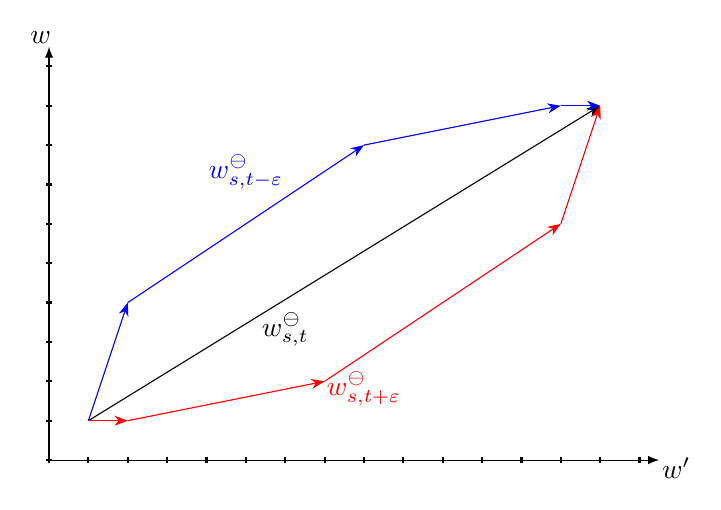
\begin{tikzpicture}[yscale=0.5,xscale=0.5]
		\tkzInit[xmin=20,ymin=12,xmax=35,ymax=22]
		\tkzDrawX[label={$w'$},right]
		\tkzDrawY[label={$w$},above]
		
		\tkzDefPoint(21,13){A}
		\tkzDefPoint(34,21){B}
		\draw[color=black,-Stealth] (A)--(B);
		
		\tkzDefPoint(26,16){U}
		\tkzLabelPoint(U){$w^{\ominus}_{s,t}$};
		
		\tkzDefPoint(22,13){C}
		\tkzDefPoint(27,14){D}
		\tkzDefPoint(33,18){E}
		\draw[color=red,-Stealth] (A)--(C);
		\draw[color=red,-Stealth] (C)--(D);
		\draw[color=red,-Stealth] (D)--(E);
		\draw[color=red,-Stealth] (E)--(B);
		\tkzDefPoint(28,14.5){V}
		\tkzLabelPoint[color=red](V){$w^{\ominus}_{s,t+\varepsilon}$};
		
		\tkzDefPoint(22,16){F}
		\tkzDefPoint(28,20){G}
		\tkzDefPoint(33,21){H}
		\draw[color=blue,-Stealth] (A)--(F);
		\draw[color=blue,-Stealth] (F)--(G);
		\draw[color=blue,-Stealth] (G)--(H);
		\draw[color=blue,-Stealth] (H)--(B);
		\tkzDefPoint(25,20){V}
		\tkzLabelPoint[color=blue](V){$w^{\ominus}_{s,t-\varepsilon}$};
		
		
		
	\end{tikzpicture}
\end{proof}

\vspace{1cm}
\begin{lemma}[monotonic $w$]
	Fixing $n$ and $s$, $w_{s,t}(n)$ contains a non-increasing function of $t$; that is, there exists a function $w^{\star}_{s,t}(n) \in w_{s,t}(n)$ that is non-increasing w.r.t. $t$
\end{lemma}
\begin{proof}
	$w^{\star}_{s,t}(n) = \lfloor w^{\ominus}_{s,t}(n)\rfloor$ is such a function.
\end{proof}

\vspace{1cm}
\begin{lemma}[Mode $M_0$] The optimizer degenerates at extreme $s/t$ ratio. For $n \geq2$
	\begin{align*}
	E_{s,t}(n) = (n-1)t + \frac{1}{2}n(n-1)s,\quad & w_{s,t}(n) = \{1\},\quad  &\text{for } \frac{t}{s} > n - 2 \\
	E_{s,t}(n) = (n-1)s + \frac{1}{2}n(n-1)t,\quad & w_{s,t}(n) = \{n-1\},\quad  &\text{for } \frac{t}{s} < \frac{1}{n-2}
	\end{align*}
\end{lemma}
\begin{proof}
	The two statements above are equivalent due to the symmetry property, so we will just prove the first one by induction
	\paragraph{Base case} For $n=2$, $w_{s,t}(2) = 1$ is the only possible choice, and
	\[
	E_{s,t}(2) = E_{s,t}(1) + E_{s,t}(1) + t + s = t + s = (2-1)t + \frac{1}{2}\cdot 2 \cdot (2-1) s
	\]
	\paragraph{Inductive step} Assuming $E_{s,t}(k) = (k-1)t + \frac{1}{2}k(k-1)s$ holds for all $k = 1,2,\dots, n-1$ and $t/s > k - 2$, we can show that, for $t/s > n - 2 > k - 2$:
	\begin{align*}
	D^w_{s,t}(n) &= E_{s,t}(w) + E_{s,t}(n-w)+wt+(n-w)s \\
	&=(w-1)t + \frac{1}{2}w(w-1)s + (n-w-1)t + \frac{1}{2}(n-w)(n-w-1)s+wt+(n-w)s\\
	&= sw^2 + (t-(n+1)s)w + (n-2)t + \frac{1}{2}n(n+1)s
	\end{align*}
	The function $D^w_{s,t}(n)$ is quadratic over $w$, which has the axis
	\[
		w_{axis} = -\frac{t-(n+1)s}{2s} = \frac{1}{2}\left(-\frac{t}{s} + n+1\right) < \frac{3}{2}
	\]
	The positive integer $w$ that's the closest to the axis gets the minimal value. We can see that $w=1$ is always the closest to the axis, therefore it minimize the function to
	\[
		E_{s,t}(n) = D^1_{s,t}(n) =s + (t-(n+1)s) + (n-2)t + \frac{1}{2}n(n+1)s = (n-1)t + \frac{1}{2}n(n-1)s
	\]
\end{proof}


\vspace{1cm}
\begin{lemma}[Mode $M_1$]  For $R = \lfloor t/s\rfloor \geq 2$, $k = 1,2,\dots,R + 2$ and  $p = 0, 1, \dots k - 1$, define
	\[
		n_{k,p} = R + \frac{1}{2}k(k-1) + 1 + p
	\]
	Then we have
	\begin{align*}
	    w_{s,t}(n_{k, 0}) &= \{k-1\} &\quad(k\geq 2, t/s\notin\mathbb{Z})\\
	    w_{s,t}(n_{k, 0}) &= \{k-1, k\} &\quad(k\geq 2, t/s\in\mathbb{Z})\\
	    w_{s,t}(n_{k, p}) &= \{k-1, k\}&\quad (k\geq 3 \text{ and } 1 \leq p\leq k-2)\\
	    w_{s,t}(n_{k, k-1}) &= \{k\}\\
	\end{align*}
	(However, if $t/s\in\mathbb{Z}$, $k=R+2$ and $p \geq 1$, the $w_{s,t}(n_{k, p})$ set could be a superset of what's listed above)
	\[
	E_{s,t}(n_{k, p}) = \left(R+(k-1)^2+2p\right)t + \left( \frac{1}{3}(k^3-3k^2+(3R+5)k+\frac{3}{2}(R+1)(R-2)) + p(k-1) \right) s
	\]
\end{lemma}
\begin{proof}

Mode $M_1$ chops the $(n, E(n))$ curve into $(R + 2)$ segments with increasing length. e.g. The first segment $S_1$ covers $n \in \{n_{1,0}\} = \{R + 1\}$, the segment $S_2$ covers $n \in \{n_{2,0},n_{2,1}\} = \{R + 2, R + 3\}$, and so on. Note that the first segment $S_1$ is inside mode $M_0$, and the second segment $S_2$ overlaps with the end of $M_0$ at the first $n$ (except for $t/s\in\mathbb{Z}$).

We will prove the property using induction.

\paragraph{Base case} Since the first segment $S_1$ is inside $M_0$, we can verify using the previous property. Indeed, we have
\begin{align*}
w(n_{1,0}) &= w(R + 1) = \{1\} \\
E(n_{1,0}) &= E(R + 1) = Rt + \frac{1}{2}R(R+1)s\\
 &= (R+(1-1)^2+2\cdot 0)t + \left( \frac{1}{3}(1^3-3\cdot1^2+(3R+5)\cdot 1+\frac{3}{2}(R+1)(R-2)) + 0\cdot(1-1) \right) s
\end{align*}
The value for $w(n)$ is irregular at $k=1$ comparing to the rest in mode $M_1$, but we won't use it in induction, so it doesn't matter.

If $t/s\notin\mathbb{Z}$, the first point of $S_2$ is also the last point of $M_0$, let's verify it:
\begin{align*}
w(n_{2,0}) &= w(R + 2) = \{1\}\\
E(n_{2,0}) &= E(R + 2) = (R+1)t+\frac{1}{2}(R+1)(R+2)s\\
&= \left(R+1^2+2\cdot0\right)t + \left( \frac{1}{3}(2^3-3\cdot 2^2+(3R+5)\cdot 2+\frac{3}{2}(R+1)(R-2)) + 0\cdot 1 \right) s
\end{align*}
This formula is actually also applicable to $t/s\in\mathbb{Z}$. However, in that case $w_{axis} = 3/2$, so we have $w(n_{2,0}) = \{1, 2\}$, but the formula for $E(n_{2,0})$ still holds.

The second point of $S_2$ is just outside $M_0$. We can continue our previous proof for $M_0$ to find the value of this point. The quadratic function $D^w(n)$ to minimize still holds (because all previous points are still in $M_0$), however its axis is now moved closer to 2:
\[
w_{axis} =  \frac{1}{2}\left(-\frac{t}{s} + n+1\right) =  \frac{1}{2}\left(-\frac{t}{s} + R+3 +1\right)\in\left(\frac{3}{2}, 2\right] \implies w(n_{2,1}) = \{2\}
\]
\begin{align*}
E(n_{2,1}) &= E(R + 3) = 4s + 2(t-(R+4)s) + (R+1)t+\frac{1}{2}(R+3)(R+4)s = (R+3)t + \left(\frac{1}{2}R^2+\frac{3}{2}R+2\right)s\\
&=\left(R+1^2+2\cdot 1\right)t + \left( \frac{1}{3}(2^3-3\cdot 2^2+(3R+5)\cdot 2+\frac{3}{2}(R+1)(R-2)) + 1\cdot 1 \right) s
\end{align*}

We have verified that the formula for $M_1$ holds for segments $S_1$ and $S_2$. In the inductive step, we will use this base to proof the formula for $S_k$ where $k \geq3$

\paragraph{Inductive step}
We assume that $E(m)$ for all $m <n$ satisfies the corresponding $M_0$ or $M_1$ formula, and we want to compute the next value $E(n)$ to verify that it also satisfies the formula. Using the property that function $E(n)$ is convex over $n$, we know that as long as we find a local minimum of $D^w(n)$, it will be the global minimum and be the value of $E(n)$.

If you don't want to use the general convexity property, here is a proof that mode $M_0$ and $M_1$ are convex. Mode $M_0$ itself is obviously convex, as it is a quadratic function over $n$. Each segment $S_k$ of $M_1$ is also obviously convex, as it is linear over $p$, which in turn is linear over $n$. We only need to prove that the ``transition" between segments are also convex. For the transition from $M_0$ to $S_2$ (we skip $S_1$ because it is inside $M_0$), we have
\begin{align*}
\Delta E(R+1) &= E(R+2) - E(R+1) = t + (R+1)s\quad&\begin{cases}
\text{(the last two points of $M_0$, $t/s\notin\mathbb{Z}$)}\\
\text{(the connecting segment between $M_0$ and $S_2$, $t/s\in\mathbb{Z}$)}
\end{cases}\\
\Delta E(R+2) &= E(R+3) - E(R+2) = 2t + s\quad&\text{(the first two points of $S_2$)}\\
\Delta E(R+1) &\leq \Delta E(R+2) \quad&\left(R = \left\lfloor\frac{t}{s}\right\rfloor \leq \frac{t}{s}\right)
\end{align*}
thus the transition from $M_0$ to $S_2$ is convex. And then for transition from $S_k$ to $S_{k+1}$, we have
\begin{align*}
\Delta E(n_{k,k-2}) &= E(n_{k,k-1}) - E(n_{k,k-2}) = 2t + (k-1)s\quad&\text{(the last two points of $S_k$)}\\
\Delta E(n_{k,k-1}) &= E(n_{k+1, 0}) - E(n_{k,k-1}) = t + (k+R)s\quad&\text{(the connecting segment)}\\
\Delta E(n_{k+1,0}) &= E(n_{k+1, 1}) - E(n_{k+1,0}) = 2t + ks\quad&\text{(the first two points of $S_{k+1}$)}\\
\Delta E(n_{k,k-2}) &<  \Delta E(n_{k,k-1}) \leq \Delta E(n_{k+1,0}) \quad&\left(\frac{t}{s} -1 < R = \left\lfloor\frac{t}{s}\right\rfloor \leq \frac{t}{s}\right)
\end{align*}
thus the transition from $S_k$ to $S_{k+1}$ is convex. We have shown that $E(m)$ for all $m<n$, assuming the formula is correct, is convex.

Now for $n = n_{k, p}$, the function to minimize $D^w(n)$ has the following differential equation
\begin{align*}
\Delta_w D^w(n) &= D^{w+1}(n)-D^w(n) \\
&= \Delta E(w) - \Delta E(n-w-1) + t -s
\end{align*}
and then let's look at the differentials between $w = k-2, k-1, k, k+1$ (remember we are discussing $k\geq3$ and $n > R + k(k-1)/2 $ so these are all valid $w$):
\begin{align*}
\Delta_w D^{k-2}(n_{k,p}) &=  \Delta E(k-2) - \Delta E(n_{k,p}-k+1) + t -s \\
&= t+(k-2)s - \begin{cases}
2t + (k-2)s\ &(0\leq p \leq k-3)\\
t + (k-1+R)s\ &(p = k-2)\\
2t + (k-1)s\ &(p = k-1)
\end{cases} + t-s\\
&\leq s \\
&< 0 \\ \\
\Delta_w D^{k-1}(n_{k,p}) &=  \Delta E(k-1) - \Delta E(n_{k,p}-k) + t -s \\
&= t+(k-1)s - \begin{cases}
t + (k-2+R)s\ &(p =0)\\
2t + (k-2)s\ &(1\leq p\leq k-2)\\
t + (k-1+R)s\ &(p = k-1)
\end{cases} + t-s\\
&= \begin{cases}
t -Rs \geq 0\ &(p =0)\\
0\ &(1\leq p \leq k-2)\\
t -(R+1)s < 0\ &(p = k-1)
\end{cases}\\ \\
\Delta_w D^{k}(n_{k,p}) &=  \Delta E(k) - \Delta E(n_{k,p}-k-1) + t -s \\
&= \begin{cases}
t+ks &(k \leq R + 1)\\
2t+s&(k = R + 2)
\end{cases} - \begin{cases}
2t + (k-3)s\ &(p =0)\\
t + (k-2+R)s\ &(p =1)\\
2t + (k-2)s\ &(2\leq p \leq k-2)\\
\end{cases} + t-s\\
&\geq \begin{cases}
s &(k \leq R + 1)\\
t-Rs&(k = R + 2)
\end{cases}\\
&\geq0 \text{ (equality holds only when $k=R+2$, $p\geq 1$ and $t/s\in\mathbb{Z}$)}
\end{align*}
Because $\Delta_w D^{k-2}(n_{k,p}) < 0 $ and $\Delta_w D^k(n_{k,p}) > 0$ (excluding $k=R+2$ and $t/s\in\mathbb{Z}$), the minimum must be among $D^{k-1}(n_{k,p})$ and $D^k(n_{k,p})$. This depends on the sign of $\Delta_w D^{k-1}(n_{k,p})$:
\[
\begin{cases}
p = 0 &\implies \Delta_w D^{k-1}(n_{k,p}) \geq 0 \implies w(n_{k,p})  = \begin{cases}\{k-1\} &(t/s\notin\mathbb{Z}) \\ \{k-1, k\} &(t/s\in\mathbb{Z})\end{cases} \\
1\leq p \leq k-2 &\implies \Delta_w D^{k-1}(n_{k,p}) = 0 \implies w(n_{k,p})  = \{k-1, k\}\\
p = k-1 &\implies \Delta_w D^{k-1}(n_{k,p}) < 0 \implies w(n_{k,p})  = \{k\}
\end{cases}
\]
For the special case $k=R+2$, $p\geq 1$ and $t/s\in\mathbb{Z}$, the $w$ values above are still valid, but because $\Delta_w D^k(n_{k,p}) = 0$, there could be more $w$ that minimizes $D^w(n)$.

Now we can calculate $E(n_{k,p})$. For $0\leq p \leq k-2$, we have
\begin{align*}
E(n_{k,p}) &= D^{k-1}(n_{k,p}) \\
&= E(k-1) + E(n_{k,p} - (k-1)) + (k-1)t + (n_{k,p} - (k-1))s\\
&=E(k-1) + E(n_{k-1,p}) + (k-1)t + n_{k-1,p}s\\
&=(k-2)t + \frac{1}{2}(k-1)(k-2)s\\ & + \left(R+(k-2)^2+2p\right)t + \left( \frac{1}{3}((k-1)^3-3(k-1)^2+(3R+5)(k-1)+\frac{3}{2}(R+1)(R-2)) + p(k-2) \right) s \\&+ (k-1)t + \left(R + \frac{1}{2}(k-1)(k-2) + 1 + p\right)s\\
&=\left(R+(k-1)^2+2p\right)t+ \left( \frac{1}{3}(k^3-3k^2+(3R+5)k+\frac{3}{2}(R+1)(R-2)) + p(k-1) \right) s
\end{align*}
and for $1\leq p \leq k-1$, we have
\begin{align*}
E(n_{k,p}) &= D^{k}(n_{k,p}) \\
&= E(k) + E(n_{k,p} - k) + kt + (n_{k,p} - k)s\\
&=E(k) + E(n_{k-1,p-1}) + kt + n_{k-1,p-1}s\\
&=(k-1)t + \frac{1}{2}k(k-1)s
\\&+\left(R+(k-2)^2+2(p-1)\right)t + \left( \frac{1}{3}((k-1)^3-3(k-1)^2+(3R+5)(k-1)+\frac{3}{2}(R+1)(R-2)) + (p-1)(k-2) \right) s
\\&+kt + \left(R + \frac{1}{2}(k-1)(k-2) + p\right)s
\\&=\left(R+(k-1)^2+2p\right)t+ \left( \frac{1}{3}(k^3-3k^2+(3R+5)k+\frac{3}{2}(R+1)(R-2)) + p(k-1) \right) s
\end{align*}

\end{proof}


\vspace{1cm}
\begin{lemma}[Fancy mode $M_1$] for $3\leq t/s +1 \leq n \leq \lfloor t/s\rfloor^2/2+5\lfloor t/s\rfloor / 2 +2$
	\begin{align*}
		w^{\min}_{s,t}(n) &= \left\lceil \sqrt{2\left(n-\frac{t}{s}\right)+\frac{9}{4}}-\frac{3}{2} \right\rceil\\
		w^{\max}_{s,t}(n) &= \left\lfloor \sqrt{2\left(n-\frac{t}{s}\right)-\frac{7}{4}}+\frac{1}{2} \right\rfloor\\
	\end{align*}
\end{lemma}

\vspace{1cm}
\begin{definition}[Continuous]
	Define the following function $\tilde{E}: [1, \infty)\to\mathbb{R}$
	\begin{align*}
		\tilde{E}_{s,t}(1) &= 0, \\
		\tilde{E}_{s,t}(n) &= \min_{0<w<n}^{w\in\mathbb{R}}\{\tilde{E}_{s,t}(w) + \tilde{E}_{s,t}(n-w) + wt+(n-w)s\}&\text{ for } n\in(1,\infty) \\
		\end{align*}
\end{definition}

\vspace{1cm}
\begin{definition}[Continuous growth rate]
	Define $\rho_{s,t}$ to be the real solution to the equation
	\[
	e^{-sr} + e^{-tr} = 1
	\]
\end{definition}


\vspace{1cm}
\begin{lemma}[Continuous]$\tilde{E}_{s,t}$ has the formula
	\[
	\tilde{E}_{s,t}(n) = \frac{n\ln n}{\rho_{s,t}}
	\]
	and $g_{s,t} =  w / n $ ($w$ being the optimizer for $\tilde{E}$) is independent from $n$ and satisifes
	\[
	\frac{\ln g}{\ln(1-g)} = \frac{t}{s}\quad\text{ or }\quad g^{s} = (1-g)^t\,.
	\]
\end{lemma}
\begin{proof}
	This is rather a heuristic observation than a concrete theorem. Guess that $\tilde{E}_{s,t}$ has the $n \ln n$ form with an unknown coefficient. Consider the derivative
	\begin{align*}
	&\frac{d}{dw} \left( \frac{w\ln w}{\rho_{s,t}}  + \frac{(n-w)\ln (n-w)}{\rho_{s,t}} +wt+(n-w)s \right)\\
	&=\frac{1 + \ln w}{\rho_{s,t}} - \frac{1 + \ln(n-w)}{\rho_{s,t}}+t-s\\
	&=\frac{\ln w - \ln (n-w)}{\rho_{s,t}} + t -s
	\end{align*}
	The derivative monotonically increases in $0<w<n$ and approaches $\pm \infty$ at each end respectively, so the single minimal value of the original function is at derivative of $0$
	\begin{align*}
	\frac{\ln w - \ln (n-w)}{\rho_{s,t}} + t -s &= 0\\
	\rho_{s,t} &= \frac{\ln w - \ln (n-w)}{s -t }
	\end{align*}
	and we substitute this back and remove the $\min$ operator, we get
	\[
	\frac{s -t }{\ln w - \ln (n-w)} n\ln n =  \frac{s -t }{\ln w - \ln (n-w)}w\ln w + \frac{s -t }{\ln w - \ln (n-w)}(n-w)\ln (n-w)+wt+(n-w)s\,,
	\]
	which can be simplified to
	\[
	\frac{\ln(w/n)}{\ln(1-w/n)} = \frac{t}{s}\,.
	\]
	With $g_{s,t} = w/n$, we have
	\[
	\frac{\ln g}{\ln(1-g)} = \frac{t}{s}\,.
	\]
	We can also get the coefficient $\rho_{s,t}$ by
	\[
	\rho_{s,t} = \frac{\ln w - \ln (n-w)}{s -t } = \frac{\ln g_{s,t} - \ln (1-g_{s,t})}{s -t } = -\frac{\ln g_{s,t}}{t}= - \frac{\ln(1-g_{s,t})}{s}
	\]
	or equivalently, $\rho_{s,t} = r$ is the real solution to the equation
	\[
	e^{-sr} + e^{-tr} = 1
	\]
\end{proof}

\vspace{1cm}
\begin{lemma}[Continuous] for all positive integer $n$
	\[
	E_{s,t}(n) \geq \tilde{E}_{s,t}(n)
	\]
\end{lemma}
\begin{proof}
	 The optimizer for $\tilde{E}$ is always in a super set for the one for $E_{s,t}$
\end{proof}

\vspace{1cm}
\begin{lemma}[$E$ limit]
	\[
	\lim_{n\to\infty}\frac{E_{s,t}(n)}{\tilde{E}_{s,t}(n)} = 1
	\]
\end{lemma}
\begin{proof}

	We will use the function $\eta(x)$ previously defined. First of all, let's show that $\eta(x)$ has asymptotic behavior
	\[
	\frac{\eta(x)}{e^{\rho_{s,t} x}} = C \in [e^{-(s+t)\rho_{s,t}},e^{-\min\{s,t\}\rho_{s,t}}]
	\]
	It is easy to show that any function in the form
	\[
	\eta'(x) = C e^{\rho_{s,t} x}
	\]
	satisfies the functional equation
	\[
	\eta'(x) = \eta'(x - s) + \eta'(x - t)
	\]
	which $\eta(x)$ also satisfies. So if we find a $\eta'(x)$ that is completely larger or smaller than $\eta(x)$ in the seeding region $(\min\{s,t\}, s+t]$, then by induction such $\eta'(x)$ will always bound $\eta(x)$ above or below. We can choose the end points of the seeding region to get $C_{hi} = e^{-\min\{s,t\}\rho_{s,t}}$ and $C_{lo} = e^{-(s+t)\rho_{s,t}}$ for the upper and lower bound.

	We then prove the limit on the sequence $\{\eta_k\}_{k=1}^{\infty}$ . We want to prove
	\[
	\lim_{k\to\infty}\frac{E_{s,t}(\eta_k)}{\tilde{E}_{s,t}(\eta_k)} = 1
	\]
	The value of $E(\eta_k)$ can be expressed as
	\begin{align*}
	E(\eta_k) &= x_1 (\eta_2 - \eta_1) + x_2 (\eta_3 - \eta_2) + \dots +x_{k-1} (\eta_k - \eta_{k-1})\\
	&=  x_{k-1}\eta_k - (x_1 \eta_1 + (x_2 - x_1) \eta_2 + (x_3 - x_2)\eta_3 + \dots + (x_{k-1} - x_{k-2}) \eta_{k-1}) \\
	&< x_{k-1}\eta_k
	\end{align*}
	We can use the squeeze theorem (Remember $E(n) \ge \tilde{E}(n)$) and only prove the following limit instead
	\[
	\lim_{k\to\infty}\frac{x_{k-1}\eta_k}{\tilde{E}_{s,t}(\eta_k)} = \lim_{k\to\infty}\frac{\rho_{s,t}x_{k-1}}{\ln\eta_k} = 1
	\]
	Recall the asymptotic behavior of $\eta(x)$, we have
	\begin{align*}
	\frac{\rho_{s,t}x_{k-1}}{\ln\eta_k} &= \frac{\rho_{s,t}x_{k-1}}{\ln\eta(x_k)} \\
	&=\frac{\rho_{s,t}x_{k-1}}{\ln\left(C e^{\rho_{s,t}x_k}\right)}\\
	&=\frac {\rho_{s,t}x_{k-1}}{\rho_{s,t}x_k +\ln C }
	\end{align*}
	The difference between $x_{k-1}$ and $x_k$ is bounded
	\[
	x_k - x_{k-1} = M \le \max\{s, t\}
	\]
	because otherwise we would have a long constant region for $\eta(x)$, which traces back to an equally long seeding region, which we know is only $\max\{s, t\}$ long. On the other hand, the sequence $\{x_k\}$ is unbounded, because each jump point at $x_k$ should create another two jump points $x_k+s$ and $x_k+t$ that is also part of the $\{x_k\}$ sequence, thus leading the sequence to grow unbounded. This means the limit
	\begin{align*}
	\lim_{k\to\infty}\frac{\rho_{s,t}x_{k-1}}{\ln\eta_k} &= \lim_{k\to\infty}\frac {\rho_{s,t}x_{k-1}}{\rho_{s,t}x_k +\ln C } \\
	&= \lim_{k\to\infty}\frac {\rho_{s,t}x_{k-1}}{\rho_{s,t}(x_{k-1} + M) +\ln C }\\
	&= \lim_{k\to\infty}\frac {1}{1 + \frac{\rho_{s,t}M +\ln C}{\rho_{s,t}x_{k-1}} } \\
	&=1
	\end{align*}
	and we therefore proved the limit on the subsequence
	\[
	\lim_{k\to\infty}\frac{E_{s,t}(\eta_k)}{\tilde{E}_{s,t}(\eta_k)} = 1
	\]

	In order to prove the full limit, let's look at some properties of $\tilde{E}(n)$. Consider the following two points on the curve
	\begin{align*}
	A &= (a, K a\ln a)\\
	B &= (b, K b\ln b)
	\end{align*}
	The tangent at $A$ has the following equation
	\[
	Y_a(n) = K(\ln a + 1)n - Ka
	\]
	Because $\tilde{E}(n)$ is convex, this tangent line is always below $\tilde{E}(n)$. We denote the linear function that passes both $A$ and $B$ as $L_{a,b}(n)$. Then for $a\le n\le b$, we have
	\begin{align*}
	\frac{L_{a,b}(n)}{\tilde{E}(n)} &\le \frac{L_{a,b}(n)}{Y_a(n)} \\
	&\le \frac{L_{a,b}(b)}{Y_a(b)} \\
	&= \frac{Kb \ln b}{K(\ln a + 1)b - Ka}\\
	&= \frac{\ln b}{\ln a + 1 - a/b}
	\end{align*}
	Now set $a = \eta_{k} = \eta(x_k)$ and $b = \eta_{k+1} = \eta(x_{k+1})$, then their ratio is
	\begin{align*}
	\frac{a}{b} &= \frac{\eta(x_k)}{\eta(x_{k+1})}\\
		&= \frac{C e^{\rho_{s,t} x_k}}{C' e^{\rho_{s,t} x_{k+1}} } \quad &(\text{Both $C$ and $C'$ are some variables in $[e^{-(s+t)\rho_{s,t}},e^{-\min\{s,t\}\rho_{s,t}}]$})\\
		&= C'' e^{\rho_{s,t}(x_k-x_{k+1})} \quad &(C'' \in [e^{-\max\{s,t\}\rho_{s,t}}, e^{\max\{s,t\}\rho_{s,t}}]) \\
		& = C'''\in [e^{-2\max\{s,t\}\rho_{s,t}}, 1] \quad & (\text{Remember $x_{k+1} - x_{k} \le \max\{s,t\}$})
	\end{align*}
	So we can the limit
	\begin{align*}
	\lim_{k\to\infty} \frac{\ln b}{\ln a + 1 - a/b} &= \lim_{k\to\infty} \frac{\ln \eta_{k+1}}{\ln \eta_{k} + 1 - \eta_{k}/\eta_{k+1}}\\
	&= \lim_{k\to\infty} \frac{\ln \eta_{k+1}}{\ln \eta_{k+1} + \ln C''' + 1 - C'''} \\
	&= \lim_{k\to\infty} \frac{1}{1 + \frac{\ln C''' + 1 - C'''}{\ln \eta_{k+1}}} \\
	&= 1 \quad (\text{$\eta_{k+1}$ is unbounded, while $C'''$ is bounded})
	\end{align*}
	and the squeeze theorem locks the limit to
	\begin{align*}
	\lim_{k\to\infty}\frac{L_{\eta_{k},\eta_{k+1}}(n)}{\tilde{E}(n)} = 1
	\end{align*}
	Now we realize that $E(n)$ is linear between $\eta_k\le n \le \eta_{k+1}$, plus the end points has the limit
	\begin{align*}
	\lim_{k\to\infty} \frac{E(\eta_k)}{\tilde{E}(\eta_k)} &= \lim_{k\to\infty} \frac{E(\eta_k)}{L_{\eta_{k},\eta_{k+1}}(\eta_k)} = 1 \\
	\lim_{k\to\infty} \frac{E(\eta_{k+1})}{\tilde{E}(\eta_{k+1})} &= \lim_{k\to\infty} \frac{E(\eta_{k+1})}{L_{\eta_{k},\eta_{k+1}}(\eta_{k+1})} = 1
	\end{align*}
	Then the two linear function has limit for any point in $\eta_k\le n \le\eta_{k+1}$
	\begin{align*}
	\lim_{k\to\infty} \frac{E(n)}{L_{\eta_{k},\eta_{k+1}}(n)} = 1 \quad(\text{arbitrarily choose a $n\in[\eta_k,\eta_{k+1}]$ for each $k$})
	\end{align*}
	Combining with the previous limit between $L$ and $\tilde{E}$, we get
	\begin{align*}
	\lim_{k\to\infty} \frac{E(n)}{\tilde{E}(n)} = 1
	\end{align*}
	which implies
	\[
	\lim_{n\to\infty} \frac{E(n)}{\tilde{E}(n)} = 1
	\]


\end{proof}

\paragraph{Remark}

The proof also hinted the function converges at the order of $1+\mathcal{O}(1/\log(n))$, which is very slow.


\vspace{1cm}
\begin{lemma}[Fibonacci asymptote]
	For coprime integer pair $(s, t)$, the genfib sequence $\{n_i\}_{i=\min\{s,t\}+1}^{\infty}$ has the following asymptotic behavior
	\[
	\lim_{i\to\infty}    \frac{n_i}{e^{\rho_{s,t} i}} = \frac{1}{( e^{\rho_{s,t}} - 1)(s e^{t\rho_{s,t}} + t e^{s\rho_{s,t}})}
	\]
\end{lemma}
\begin{proof}
	Remember the genfib sequence can be expressed as
	\[
	n_i = \sum_{\xi} \frac{\xi^i}{(\xi - 1)(s \xi^t + t \xi^s)}
	\]
	where $\xi$ are the complex roots of the equation
	\[
	\xi^{-s} + \xi^{-t} = 1
	\]
	All roots of this equation satisfy
	\[
	|\xi|^{-s} + |\xi|^{-t} \ge 1 \quad \text{(Triangle inequality)}
	\]
	Consider the real function $f(u) = u^{-s} + u^{-t} - 1$, which monotonically decreases and has a single root in $\mathbb{R}^+$, so the largest $u$ that satisfies $f(u)\ge 0$ is the root $u_*$ itself. Going back to $|\xi_*| = u_*$. Obviously the real value $\xi_* = u_*$ is a root of the $\xi$ equation. We can also assert that no other roots $\xi$ has the same largest magnitude  $|\xi| = u_*$, because
	\begin{align*}
	&\xi = u_*e^{i\theta} \text{ is a root} \\
	\implies& e^{-i s\theta}, e^{-i t\theta} \in \mathbb{R}^+ \quad &\text{(Triangle inequality)} \\
	\implies& s\theta, t\theta \in 2\pi\mathbb{Z} \\
	\implies& \theta \in 2\pi\mathbb{Z} \quad &(s, t \text{ coprime})\\
	\implies& \xi = u_*
	\end{align*}
	This means the original equation for $\xi$ has a single positive real root $\xi_*$, and it has the strictly largest magnitude among all complex roots. Notice that $\xi_* = e^{\rho_{s,t}}$ is a real root, so it is the root with the largest magnitude. This means that all $\lim_{i\to\infty} (\xi/\xi_*)^i$ vanishes for $\xi\ne\xi_*$, and
	\begin{align*}
	\lim_{i\to\infty}    \frac{n_i}{e^{\rho_{s,t} i}} &= \lim_{i\to\infty} \sum_{\xi} \frac{(\xi / \xi_*)^i}{(\xi - 1)(s \xi^t + t \xi^s)} \\
	&=\frac{1}{(\xi_* - 1)(s \xi_*^t + t \xi_*^s)} \\
	&=\frac{1}{( e^{\rho_{s,t}} - 1)(s e^{t\rho_{s,t}} + t e^{s\rho_{s,t}})}
	\end{align*}

\end{proof}

\vspace{1cm}
\begin{definition}[$\eta$ variation]
Define function $\upsilon_{s,t}(x)$ as
\[
\upsilon_{s,t}(x) =  \eta_{s,t}(x) \big/ \frac{e^{\rho_{s,t} x}}{\rho_{s,t}(s e^{t\rho_{s,t}} + te^{s\rho_{s,t}})}
\]
\end{definition}


\vspace{1cm}
\begin{lemma}[$\eta$ asymptote, rational]
	For $s/t\in\mathbb{Q}$, let $\kappa_{s,t} = \rho_{s,t} \gcd(s, t)$, then
	\begin{align*}
	\limsup_{x\to\infty} \upsilon_{s,t}(x) &= \frac{\kappa_{s,t}}{1 - e^{-\kappa_{s,t}}} \\
	\liminf_{x\to\infty} \upsilon_{s,t}(x) &= \frac{\kappa_{s,t}}{e^{\kappa_{s,t}} - 1}
	\end{align*}
\end{lemma}
\begin{proof}
	Let's first consider coprime integer pair $s$ and $t$ (so $\gcd(s, t) = 1$). We have previously shown the asymptotic behavior of its genfib sequence. Because $s$ and $t$ are coprime, every integer $x \ge st + s + t$ is a jump point (because such integer can always be expressed by $x = ps+qt$ with positive integers $p$ and $q$). So the $\liminf$ behavior of $ \upsilon_{s,t}(x)$ can be described by $n_x$, which are all the lower points of each jump point
	\begin{align*}
	\liminf_{x\to\infty} \upsilon_{s,t}(x) = \frac{\rho_{s,t}}{e^{\rho_{s,t}} - 1} \lim_{x\to\infty} n_x  \big/ \frac{e^{\rho_{s,t} x}}{( e^{\rho_{s,t}} - 1)(s e^{t\rho_{s,t}} + t e^{s\rho_{s,t}})}  = \frac{\rho_{s,t}}{e^{\rho_{s,t}} - 1}
	\end{align*}
	Similarly, the $\limsup$ behavior of $ \upsilon_{s,t}(x)$ can be described by $n_{x+1}$, which are all the lower points of each jump point
	\begin{align*}
	\limsup_{x\to\infty} \upsilon_{s,t}(x) = \frac{\rho_{s,t}}{e^{\rho_{s,t}} - 1} \lim_{x\to\infty} n_{x+1}  \big/ \frac{e^{\rho_{s,t} x}}{( e^{\rho_{s,t}} - 1)(s e^{t\rho_{s,t}} + t e^{s\rho_{s,t}})}  = \frac{\rho_{s,t}}{1 - e^{-\rho_{s,t}}}
	\end{align*}

	Now let's generalize this to all $s/t\in\mathbb{Q}$. First of all, we have the following identity for homogeneity
	\begin{align*}
	\eta_{ks,kt}(kx) &= \eta_{s, t}(x) \\
	k\rho_{ks,kt} &= \rho_{s,t}
	\end{align*}
	and for $\upsilon_{s,t}(x)$, we have
	\begin{align*}
	\upsilon_{ks,kt}(kx) &= \eta_{ks,kt}(kx) \big/ \frac{e^{\rho_{ks,kt} kx}}{\rho_{ks,kt}(ks e^{kt\rho_{ks,kt}} + kte^{ks\rho_{ks,kt}})} \\
		&= \eta_{s,t}(x) \big/ \frac{e^{\rho_{s,t} x}}{\rho_{s,t}(s e^{t\rho_{s,t}} + te^{s\rho_{s,t}})}\\
		&= \upsilon_{s,t}(x)
	\end{align*}
    Notice that every $(s,t)$ pair is proportional to some coprime integer pair $(s', t')$ as
	\[
	 (s,t) = \gcd(s,t)\cdot(s',t')
	\]
	so we have
	\begin{align*}
	\limsup_{x\to\infty} \upsilon_{s,t}(x) &= \limsup_{x\to\infty} \upsilon_{\gcd(s,t)s',\gcd(s,t)t'}(x) \\
	&= \limsup_{x\to\infty} \upsilon_{s',t'}\left(\frac{x}{\gcd(s,t)}\right)\\
	&= \frac{\rho_{s',t'}}{1 - e^{-\rho_{s',t'}}}\\
	&= \frac{\kappa_{s,t}}{1 - e^{-\kappa_{s,t}}}\\
	\liminf_{x\to\infty} \upsilon_{s,t}(x) &= \liminf_{x\to\infty} \upsilon_{\gcd(s,t)s',\gcd(s,t)t'}(x) \\
	&= \liminf_{x\to\infty} \upsilon_{s',t'}\left(\frac{x}{\gcd(s,t)}\right)\\
	&= \frac{\rho_{s',t'}}{e^{\rho_{s',t'}} - 1}\\
	&= \frac{\kappa_{s,t}}{e^{\kappa_{s,t}} - 1}
	\end{align*}

\end{proof}

\vspace{1cm}
\begin{lemma}[$\eta$ asymptote, irrational]
	For $s/t\notin\mathbb{Q}$
	\begin{align*}
	\lim_{x\to\infty} \upsilon_{s,t}(x) = 1
	\end{align*}
\end{lemma}
\begin{proof}
First, let's observe the properties of the roots $r$ of the equation
\[
e^{-sr} + e^{-tr} = 1
\]
We already introduced a real root of this equation $\rho$. In fact, we can show that $\rho$ has uniquely the largest real component among all complex roots when $s/t\notin\mathbb{Q}$: all roots satisfies the triangle inequality
\[
|e^{-sr}| + |e^{-tr}| = e^{-s\Re(r)} + e^{-t\Re(r)} \ge 1
\]
Because the left side is a decreasing function of $\Re(r)$, we have $\Re(r) \le \rho$. Let's assume there is another root $r=\rho + i\theta$ with the same real component, then the triangle inequality requires
\begin{align*}
e^{-is\theta},e^{-it\theta}\in\mathbb{R^+}\implies  s\theta,t\theta\in2\pi\mathbb{Z}
\end{align*}
which is only possible for $\theta = 0$ due to irrational $s/t$.

On the other hand, all roots $r$ are bounded on the left side as well. For $r$ with low enough real component, $|e^{-sr} + e^{-tr}| \ge |e^{-s\Re(r)} - e^{-t\Re(r)}|$ can grow unbounded, nullifying the possibility of a root which would require  $|e^{-sr} + e^{-tr}|=1$.

We can also show that all complex roots is distributed evenly. Let's consider a rectangular contour on $g(r) = e^{-sr} + e^{-tr} - 1$ for the argument principle, whose height is $H$, and the left and right sides are far away enough. For the top and the bottom sides, as only $\Re(r)$ changes, the total change in $\Arg(g(r))$ is less than $2\pi$. For the right side, because $g(r)$ is always very close to $-1$, the total change in $\Arg(g(r))$ is also less than $2\pi$. For the left side, $g(r)$ is asymptotically similar to $e^{-\max\{s,t\}r}-1$, which has total change in $\Arg(g(r))$ of about $\max\{s,t\}H$. So in general, the total number of roots inside the contour is about $\max\{s,t\}H/(2\pi)$, give or take 3. Because all roots are also restricted in a vertical strip, we can show that
\[
\lim_{n\to\infty}\frac{|r_n|}{n} = \frac{\pi}{\max\{s,t\}}
\]
where $r_n$ are roots in ascending order in their magnitude.

Next, let's introduce the smooth step function, for a small positive $\mu$
\[
\theta^{\mu}(x) = \begin{cases}
0 \quad &(x < 0) \\
\frac{x}{\mu} \quad &(0\le x\le \mu)\\
1 \quad &(x>\mu)
\end{cases}
\]
which has Laplace transform
\begin{align*}
\mathcal{L}\{\theta^{\mu}\}(\sigma) &= \int_0^{\mu} \frac{x}{\mu} e^{\sigma x} dx + \int_{\mu}^\infty e^{\sigma x} dx = \frac{1 - e^{\mu\sigma}}{\mu\sigma^2}
\end{align*}
We can also see that
\[
	\theta^{\mu}(x)\le\theta(x)\le\theta^{\mu}(x+\mu)
\]
which is the core inequality we will build on.

Similar to the previously discussed function $\phi(x)$, we can construct its smooth version
\[
\phi^{\mu}(x) = 1 + \sum_{p=0}^{\infty}\sum_{q=0}^{\infty}\frac{(p+q)!}{p!q!}\theta^{\mu}(x-(ps+qt))
\]
which has Laplace transform
\begin{align*}
\mathcal{L}\{\phi^{\mu}\}(\sigma) &= \frac{1}{\sigma} + \frac{1-e^{-k\sigma}}{k\sigma^2(1-(e^{-s\sigma} + e^{-t\sigma}))}
\end{align*}
and by comparing coefficient at poles, we get
\begin{align*}
\phi^{\mu}(x) = \sum_{r} \frac{(1-e^{-\mu r})e^{rx}}{\mu r^2(se^{-sr}+te^{-tr})}
\end{align*}
We also inherit the inequality
\[
\phi^{\mu}(x)\le\phi(x)\le\phi^{\mu}(x+\mu)
\]

Let's explore the asymptotic behavior of $\phi^{\mu}(x)$. Consider the following limit
\begin{align*}
\lim_{x\to\infty}\frac{\phi^{\mu}(x)}{e^{\rho x}} = \lim_{x\to\infty}\sum_{r} \frac{(1-e^{-\mu r})e^{(r-\rho)x}}{\mu r^2(se^{-sr}+te^{-tr})}
\end{align*}
Let's try exchanging the limit and the summation using Tannery's theorem. We can construct the bound $M_r$
\[
M_r = \frac{U}{\mu |r|^2 V}\ge \left| \frac{1-e^{-\mu r}}{\mu r^2(se^{-sr}+te^{-tr})} \right| \ge \left| \frac{(1-e^{-\mu r})e^{(r-\rho)x}}{\mu r^2(se^{-sr}+te^{-tr})} \right|
\]
where the constants are chosen such that
\begin{itemize}
	\item $U \ge |1-e^{-\mu r}|$. $U$ exists because $\Re(r)$ is bounded on the left side, hence the the whole term is bounded in magnitude.
	\item $0 < V \le |se^{-sr}+te^{-tr}|$. To show the existence of $V$, consider $p = se^{-sr}+te^{-tr}$, which can be transformed as
	\begin{align*}
	&p = (s-t)e^{-sr} + t = (t-s)e^{-tr} + s\\
	\implies& \frac{p-t}{s-t} = e^{-sr}, \quad \frac{p-s}{t-s} = e^{-tr}\\
	\implies& \left|\frac{p-t}{s-t}\right|^t = \left|\frac{p-s}{s-t}\right|^s
	\end{align*}
	Viewed on the Cartesian plane, $p$ is on an oval-shape curve defined by the equation above. It can be seen that $0$ is not on the curve, nor its neighborhood. This means $|p|$ is lower bounded by a non-zero value.
\end{itemize}
Because of the even distribution of roots we previously showed
\[
	\lim \frac{M_r}{1/n^2} = \frac{U \max\{s,t\}^2}{\mu V \pi^2}
\]
As $\sum 1/n^2$ converges, the limit comparison test shows that the sum of all bounds converges
\[
\sum_{r} M_r < \infty
\]
This allows us to exchange the operators
\[
\lim_{x\to\infty}\frac{\phi^{\mu}(x)}{e^{\rho x}} =\sum_{r}  \lim_{x\to\infty}\frac{(1-e^{-\mu r})e^{(r-\rho)x}}{\mu r^2(se^{-sr}+te^{-tr})} = \frac{1-e^{-\mu \rho}}{\mu \rho^2(se^{-s\rho}+te^{-t\rho})}
\]

Let's go back to the inequality, and take limit on both sides
\begin{align*}
\phi^{\mu}(x)&\le\phi(x)\le\phi^{\mu}(x+\mu) \\
\frac{\phi^{\mu}(x)}{e^{\rho x}}&\le\frac{\phi(x)}{e^{\rho x}}\le e^{\mu\rho} \frac{\phi^{\mu}(x+\mu)}{e^{\rho (x+\mu)}} \\
\lim_{x\to\infty}\frac{\phi^{\mu}(x)}{e^{\rho x}} &\le \liminf_{x\to\infty}\frac{\phi(x)}{e^{\rho x}} \le \limsup_{x\to\infty}\frac{\phi(x)}{e^{\rho x}}\le e^{\mu\rho} \lim_{x\to\infty}\frac{\phi^{\mu}(x+\mu)}{e^{\rho (x+\mu)}} \\
 \frac{1-e^{-\mu \rho}}{\mu \rho}\frac{1}{\rho(se^{-s\rho}+te^{-t\rho})} &\le \liminf_{x\to\infty}\frac{\phi(x)}{e^{\rho x}} \le \limsup_{x\to\infty}\frac{\phi(x)}{e^{\rho x}}\le  \frac{e^{\mu \rho}-1}{\mu \rho}\frac{1}{\rho(se^{-s\rho}+te^{-t\rho})}
\end{align*}
Because the choice of $\mu$ is arbitrary, we can squeeze the limit
\begin{align*}
 \sup_{\mu}\frac{1-e^{-\mu \rho}}{\mu \rho}\frac{1}{\rho(se^{-s\rho}+te^{-t\rho})} &\le \liminf_{x\to\infty}\frac{\phi(x)}{e^{\rho x}} \le \limsup_{x\to\infty}\frac{\phi(x)}{e^{\rho x}}\le \inf_{\mu}\frac{e^{\mu \rho}-1}{\mu \rho}\frac{1}{\rho(se^{-s\rho}+te^{-t\rho})}\\
\frac{1}{\rho(se^{-s\rho}+te^{-t\rho})} &\le \liminf_{x\to\infty}\frac{\phi(x)}{e^{\rho x}} \le \limsup_{x\to\infty}\frac{\phi(x)}{e^{\rho x}}\le \frac{1}{\rho(se^{-s\rho}+te^{-t\rho})}
\end{align*}
\[
\lim_{x\to\infty} \frac{\phi(x)}{e^{\rho x}} = \frac{1}{\rho(se^{-s\rho}+te^{-t\rho})}
\]
which means
\begin{align*}
\lim_{x\to\infty} \nu(x) &= \lim_{x\to\infty}  \frac{e^{\rho x}}{\eta(x)\rho(se^{t\rho} + te^{s\rho})} \\
&= \lim_{x\to\infty}  \frac{e^{\rho x}}{\phi(x-s-t)\rho(se^{t\rho} + te^{s\rho})} \\
&= 1
\end{align*}
\end{proof}
\paragraph{Remark}

We could try taking the limit directly on the expansion of $\eta(x)$. However, the Tannery's theorem cannot be applied to it, because the series for $\eta(x)$ doesn't converge absolutely. This is why we went to find a pair of bounding functions whose expansion does converge absolutely, and derive the limit with squeezing method.

If we extend $\gcd$ to irrational pairs so that $\gcd(s, t) = 0$ for $s/t\notin \mathbb{Q}$, then this property can be merged with the previous property: define $\kappa_{s,t} = \rho_{s,t} \gcd(s, t)$, and $\Upsilon(x) = x/(e^x-1)$ with singularity at $x=0$ removed, then
\begin{align*}
	\limsup_{x\to\infty} \upsilon_{s,t}(x) &= e^{\kappa_{s,t}}\Upsilon(\kappa_{s,t}) \\
	\liminf_{x\to\infty} \upsilon_{s,t}(x) &= \Upsilon(\kappa_{s,t})
\end{align*}

\vspace{1cm}
\begin{definition}[$w$ deviation]
	Define the ``$w$-deviation" as
	\[
	V_{s,t}(n) = \min_{w_{s,t}^{\min}(n)\le w \le w_{s,t}^{\max}(n)}^{w\in\mathbb{R}} \left\{ \left|\frac{w}{n} - g_{s,t}\right| \right\}
	\]
\end{definition}

\vspace{1cm}
\begin{lemma}[$w$ limit]
	\[
	\lim_{n\to\infty} V_{s,t}(n) = 0
	\]
\end{lemma}
\begin{proof}
	We will first prove the following weaker limit: for jump points $\{(x_i, \eta_i\nearrow\eta_{i+1})\}_{i=1}^\infty$,
	\[
	\lim_{i\to\infty} \frac{\eta(x_i - t)}{\eta_i} = g_{s,t}
	\]

	For $s/t\in\mathbb{Q}$, without loss of generality, we will only discuss for coprime integer pair $(s, t)$. We previously proved that, for genfib sequence
	\[
	\lim_{i\to\infty}    \frac{n_i}{e^{\rho_{s,t} i}} = \frac{1}{( e^{\rho_{s,t}} - 1)(s e^{t\rho_{s,t}} + t e^{s\rho_{s,t}})}
	\]
	so we have the following limit
	\begin{align*}
	\lim_{i\to\infty} \frac{\eta(x_i - t)}{\eta_i} = \lim_{i\to\infty} \frac{n_{i-t}}{n_i}= e^{-t\rho_{s,t}}	= g_{s,t}
	\end{align*}

	For $s/t\notin\mathbb{Q}$, with the $\eta$ asymptote for irrational case
	\[
	\lim_{i\to\infty} \frac{\eta(x_i - t)}{\eta_i} = \lim_{i\to\infty} \frac{e^{\rho(x_i-t)}}{e^{\rho x_i}}  = g_{s,t}
	\]

	Remember $w_{s,t}(\eta_i) = \{\eta(x_i - t)\}$, so the limit above is actually a subsequence of the general $w$-limit at joints:
	\[
	\lim_{i\to\infty} V_{s,t}(\eta_i) = 0
	\]
	Now consider $\eta_i\le n \le \eta_{i+1}$. Because of the parallelogram property, we know that the linear interpolation $w^{\ominus}$ is within the $w$ interval
	\[
		w^{\ominus}(n) = \frac{\eta_{i+1} - n}{\eta_{i+1} - \eta_{i}} w(\eta_i) + \frac{n - \eta_{i}}{\eta_{i+1} - \eta_{i}} w(\eta_{i+1}) \in [w^{\min}(n), w^{\max}(n)]
	\]
	so we have
	\[
	V(n) \le \left|\frac{w^{\ominus}(n)}{n} - g\right|
	\]
	On the other hand, $w^{\ominus}(n)/n$ is also a linear interpolation of the joints (with a different set of parameters)
	\[
	\frac{w^{\ominus}(n)}{n} = \frac{\eta_{i+1}/n-1}{\eta_{i+1}/\eta_i-1} \frac{w(\eta_i)}{\eta_i} + \frac{\eta_{i+1}/\eta_i - \eta_{i+1}/n}{\eta_{i+1}/\eta_i-1} \frac{w(\eta_{i+1})}{\eta_{i+1}}
	\]
	so it can't be farther from $g$ than the joints are
	\[
	\left|\frac{w^{\ominus}(n)}{n} - g\right| \le \max\{ V(\eta_i), V(\eta_{i+1}) \}
	\]
	this means non-joint $V(n)$ is always bounded by joints. For $\eta_i\le n \le \eta_{i+1}$
	\[
	V(n) \le \max\{ V(\eta_i), V(\eta_{i+1}) \}
	\]
	Since the joints satisfies the limit, all points bounded by joints will satisfy the limit.
	\[
	\lim_{n\to\infty} V_{s,t}(n) = 0
	\]
\end{proof}





\vspace{1cm}
\begin{lemma} [Modes]
	The optimizer $w_{s,t}(n)$ forms several regions of ``modes" for different combination of ${n,s,t}$
\end{lemma}
\begin{proof}
	We can plot the graph of real optimizer $w_{s,t}(n)$ as a map over $n$ and $t/s$. In the following graphs, the horizontal axis from left to right is $n$ running from $2$ to $10,000,000$ in logarithmic scale, and the vertical axis from up to down is ratio $r= t/s$ running from $1$ to $10,000,000$ in logarithmic scale.  All of these graphs are expected to have a perfect mirror for $r= t/s \in (0, 1]$ in logarithmic scale so we omitted that part. These graphs aren't accurate as they don't show the values when $r$ is an integer or a simple fraction, where $w$ can be a much larger set than its neighbors; nonetheless, they still display interesting properties for most $r$.

	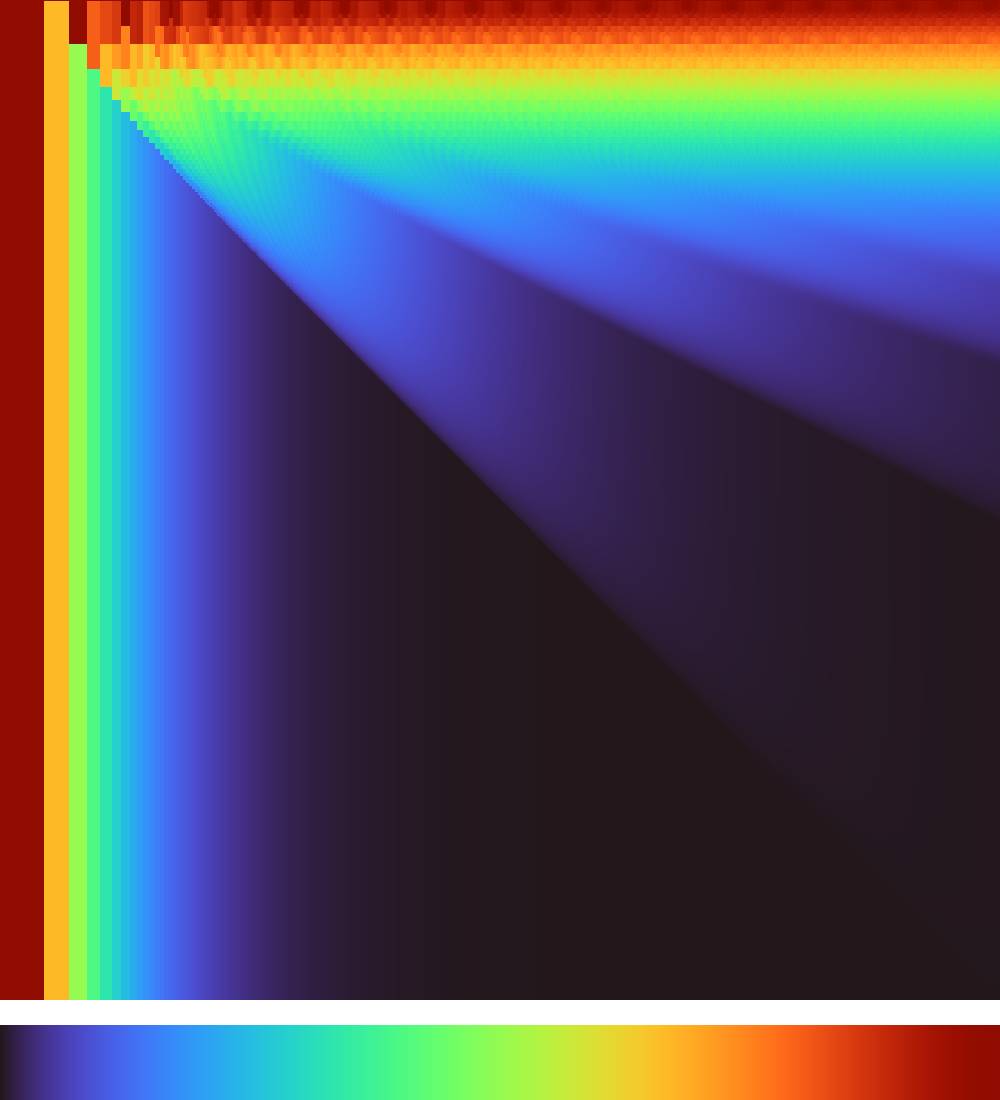
\includegraphics[scale=0.3]{w.png}\,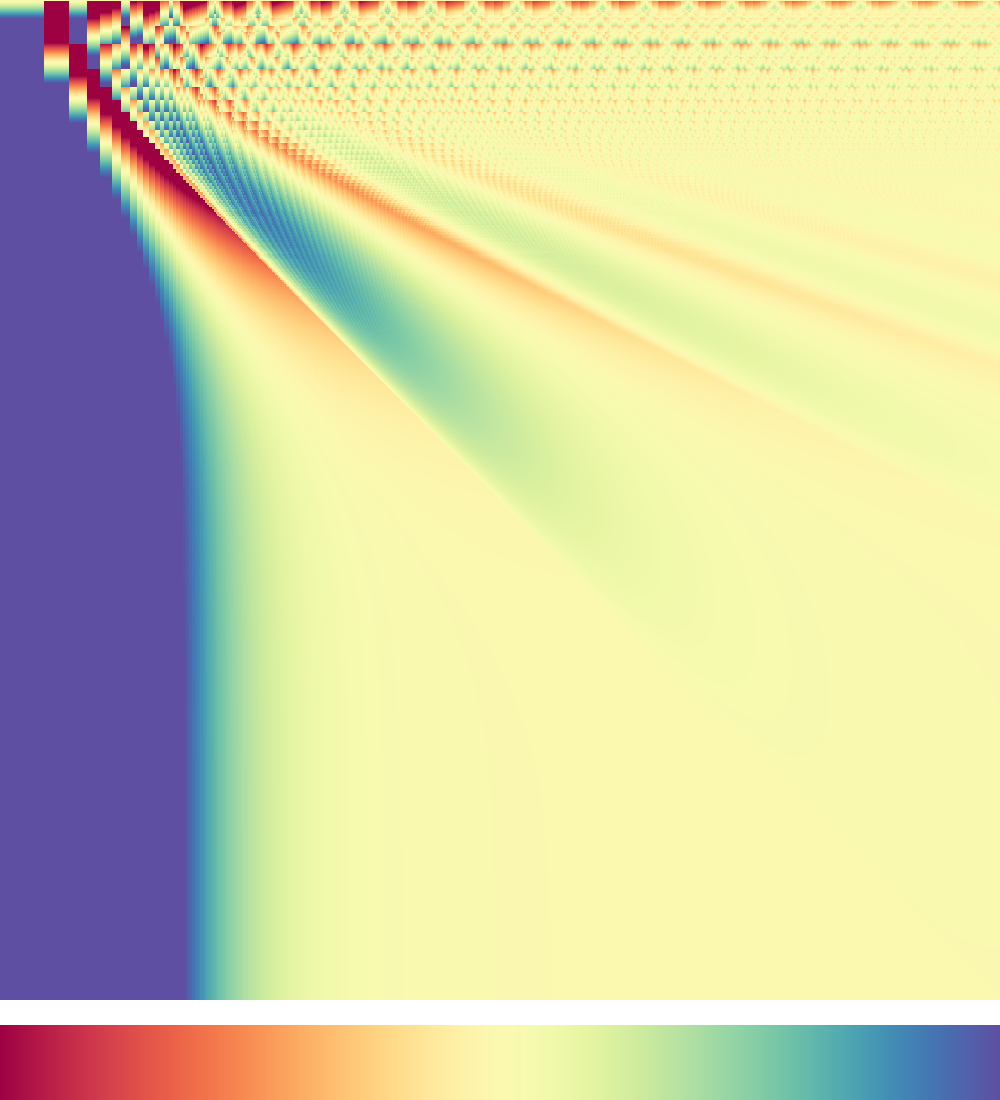
\includegraphics[scale=0.3]{bias.png}

	\vspace{0.3cm}

	
\includegraphics[scale=0.3]{variance.png}\,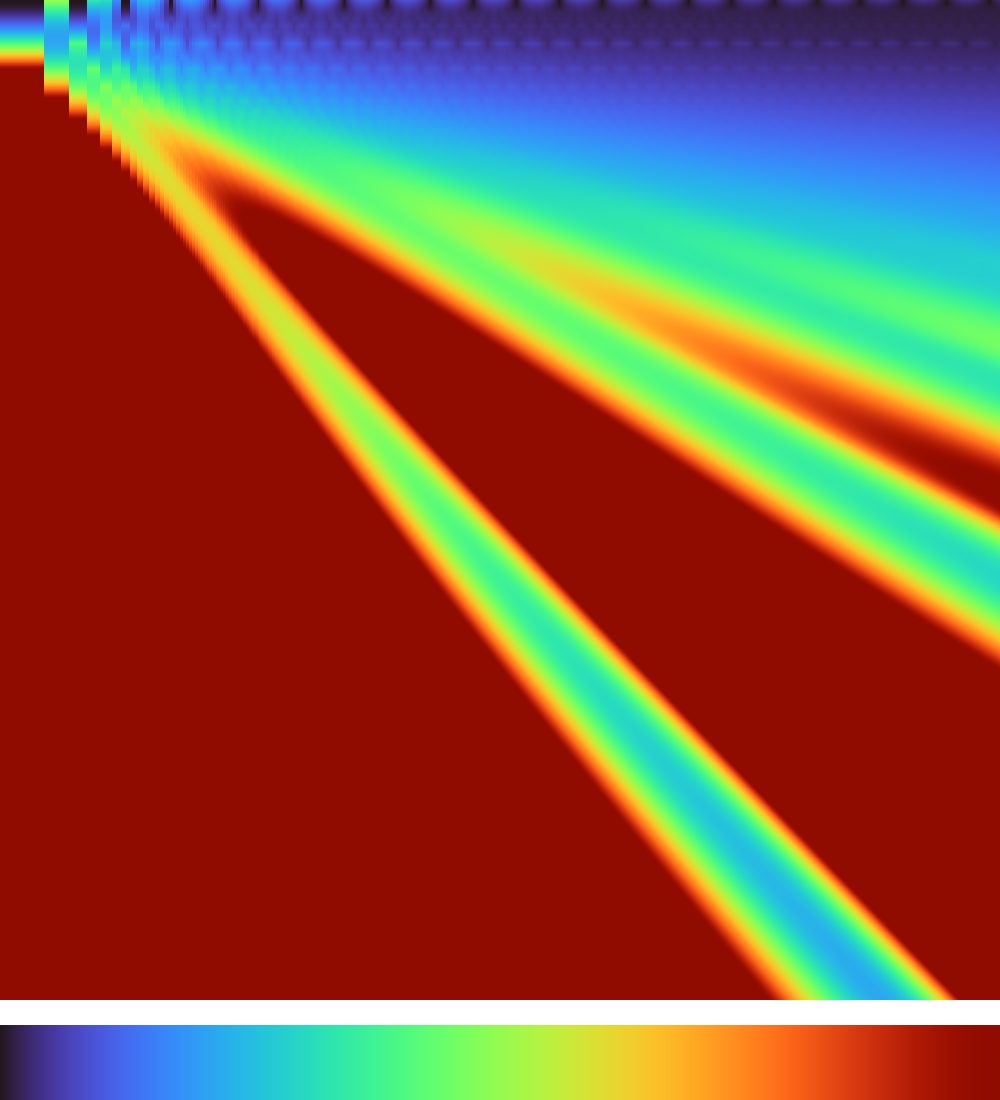
\includegraphics[scale=0.3]{e-bias.png}

	\vspace{0.3cm}

	The first graph is colored using the average relative optimizer $w_{s,t}(n)$, where color gradients runs from 0.0 to 0.5
	\[
	c_1 = \frac{w^{\max}_{s,t}(n) + w^{\min}_{s,t}(n)}{2n}
	\]
	The second graph is colored using the relative difference of optimizer $w_{s,t}(n)$ against the continuous optimizer, where 0 difference is light yellow:
	\[
	c_2 = \frac{w^{\max}_{s,t}(n) + w^{\min}_{s,t}(n)}{2n} - g_{s,t}
	\]
	The third graph is colored using the relative variance of optimizer $w_{s,t}(n)$, where 0 is colored dark green.
	\[
	c_3 = \frac{w^{\max}_{s,t}(n) - w^{\min}_{s,t}(n)}{n}
	\]
	The forth graph is colored using the relative difference between $E(n)$ and its continuous version, where dark blue means little difference, while dark red means $E(n)$ is significantly higher
	\[
	c_4 =\frac{E_{s,t}(n)} {\tilde{E}_{s,t}(n)} = \frac{\rho_{s,t} E_{s,t}(n)} {n \ln n}
	\]

	We can see the graph is divided into several regions. We have already discussed mode $M_0$ and $M_1$ above. There are also mode $M_2$, $M_3$ and so on. A new mode $M_{n+1}$ is formed when the ``short branch" ($E(w)$ when $w$ is small) falls into mode $M_n$. For mode beyond $M_4$, they seems to ``fade away" and becomes very close to the continuous optimizer. We can find the boundaries between these modes using the joint function $\eta(x)$. Consider the differential in mode $M_0$ (again we assume $t>s$)
	\[
	\Delta E(n) = t + ns, \quad n < \frac{t}{s} + 1
	\]
	which has limit
	\[
	\Delta E(n) < 2t + s
	\]
	This means the boundary between $M_0$ and $M_1$ is at
	\[
	n_{0|1} = \eta_{s,t}(2t + s)
	\]
	Because each boundary generates the next boundary by being the short branch, we can derive that in general
	\[
	n_{k|k+1} = \eta_{s,t}((k+2)t + s)
	\]
	When $t>>s$, the recurrent formula for $\eta(x)$ is similar to performing integration to previous regions. $\eta(x)$ function behaves like a linear function before $n_{0|1}$, quadratic function before $n_{1|2}$, then cubic before $n_{2|3}$, and so on. We can therefore approximate the mode boundary as
	\[
	n_{k|k+1} \sim \frac{(t/s)^{k+1}}{(k+1)!}
	\]
	Around the range where $s/t$ is close to $1$, modes seem to blend together to form the $S$ mode. This mode roughly has the boundary $n_S = e^{t/s}$. Indeed, the approximated boundary for mode $M$ always wraps around the boundary for mode $S$
	\[
	\frac{(t/s)^{k+1}}{(k+1)!} < e^{t/s}
	\]

	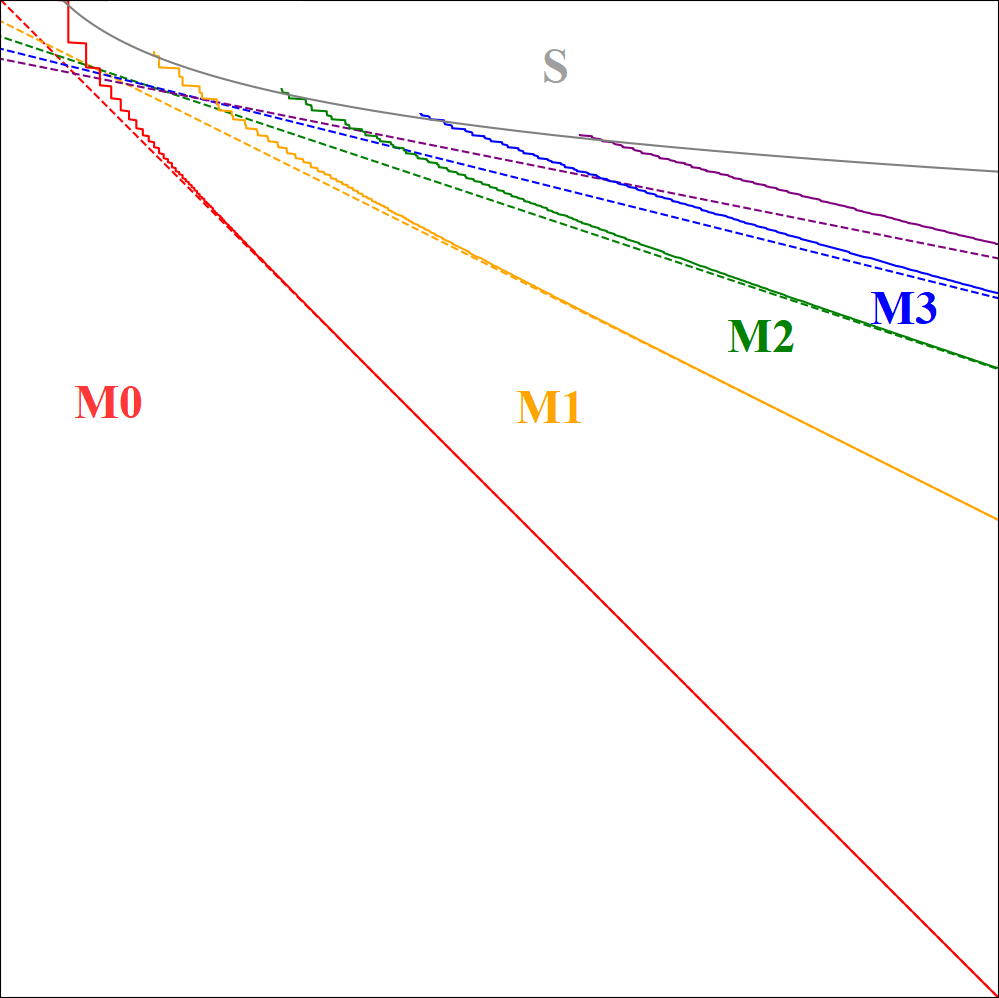
\includegraphics[scale=0.3]{mode.png}

	If we group all $n = \eta_{s,t}(ps + qt)$ by integer pairs $(p, q)$, we can get a nice pattern. In the graph below, each block in the range
	\[
	\eta_{s,t}(ps + qt) < n < \eta_{s,t}((ps + qt)^+)
	\]
	is colored according to $(p, q)$. The hue is controlled by $p$, while the brightness alternates for different $q$.

	
\includegraphics[scale=0.3]{web.png}

	This graph displays a similar pattern seen in the optimizer variance graph, and also clearly shows different regions with different colors.
\end{proof}

\vspace{1cm}
\begin{lemma} [Secondary cost]
We can extent $s$ and $t$ to any positive element in a linearly ordered albelian group.
\end{lemma}
\begin{proof}

In the proof for nodes, we used dual numbers for $s$ and $t$. This hints that the problem itself can be extended beyond real numbers. Indeed, the definition for the function $E_{s,t}(n)$ and $w_{s,t}(n)$ is well-defined for any $s$ and $t$ in a linearly ordered albelian group, where $n$ and $w$ are still positive integers, and multiplication is defined as repeated group operation.

According to Hahn embedding theorem, such group can always be embedded in some additive group $\mathbb{R}^\Psi$ endowed with a lexicographical order, where the index set $\Psi$ is well-ordered. In the previous example, dual numbers can be seen as $\mathbb{R}^{\{1, \epsilon \}} \cong \mathbb{R}\times\mathbb{R}$. In general, we can separate the group as $\mathbb{R}^\Psi \cong \mathbb{R}\times\mathbb{S}$, where $\mathbb{R}$, which we call the primary cost, is the most significant term in the lexicographical order, and $\mathbb{S}$ is the rest of the terms, which we call the secondary cost. Secondary cost has practical meaning: aside from the time cost, performing computer reboot can also cost other things such as wearing on hardware. When the time costs are equal, we might start comparing these secondary costs and have preference among options having the same primary cost.

We will use $s^\circ$ and $t^\circ$ to represent the primary cost component of $s$ and of $t$. We will also assume that both $s^\circ$ and $t^\circ$ are both positive for now. 

We can see that the many formula we have developed can be extended to $\mathbb{R}^\Psi$. For example, the $\eta(x)$ function retains its definition, only to extent its domain to $\{x\in\mathbb{R}^\Psi \,|\, x > \min\{s, t\}\}$. The set $\Omega_{s,t}^w$ also generates beads of the same size as before, and beads are still sorted by $ps+qt$. What is potentially changed is that previously merged beads due to equal $ps+qt$ can be broken up because of unequal secondary cost.

Previously we said that $w_{s,t}(n)$ only depends on the ratio $s/t$. This ratio is not well defined for an arbitrary group. We can redefine it here as follows
\begin{itemize}
	\item When $s^\circ / t^\circ$ is irrational, we define $s/t =  s^\circ / t^\circ$. In this case, the generated $w_{s,t}(n)$ purely depends on the primary cost, and is identical to $w_{s^\circ, t^\circ}(n)$. This is because all $ps+qt$ are distinct for irrational $s/t$ (hence no merged beads), and are in the same order regardless of the presence of secondary costs.
	\item When $s^\circ / t^\circ = S/T$ is rational ($S$ and $T$ are coprime positive integers), and $Ts = St$, then we define $s/t = s^\circ/t^\circ$. In this case, all secondary cost display the same ratio as the primary cost, and the generated $w_{s,t}(n)$ is identical to $w_{s^\circ, t^\circ}(n)$
	\item When $s^\circ / t^\circ = S/T$ is rational, but $Ts > St$, we define $s/t = (s^\circ/t^\circ)^+$, which is not exactly a real number. In this case, the resulting $w_{s,t}(n)$ is almost the same as $w_{s^\circ, t^\circ}(n)$, but all the merged beads break up in a way favoring using less ``$s$", identical to $w_{s^\circ+\epsilon, t^\circ}(n)$.
	\item When $s^\circ / t^\circ = S/T$ is rational, but $Ts < St$, we similarly define $s/t = (s^\circ/t^\circ)^-$. In this case, $w(n)$ is generated  identical to $w_{s^\circ-\epsilon, t^\circ}(n)$.
\end{itemize}
We have redefined $s/t$ in a set $\mathbb{R}^\star$ that extends the set of positive real numbers. $\mathbb{R}^\star$ contains all positive real numbers, but for every rational number $a$, it also adds two additional elements $a^-$ and $a^+$. These new elements capture the new equivalent classes where $s/t$ is ``almost rational", but shifted by secondary costs.

As for edge cases we haven't discussed yet:
\begin{itemize}
	\item if one of $s^\circ$ or $t^\circ$ is zero, then $w(n)$ are generated as if $s$ or $t$ is 0.
	\item if both $s^\circ$ and $t^\circ$ are zero, we can consider the next significant term in the secondary cost, and make it the new primary cost. We can then discuss according to different cases like above.
\end{itemize}	
	
\end{proof}

\vspace{1cm}
\begin{lemma}[Mode $M_0'$] If $s$ or $t$ is not a positive number, even without practical meaning, we can show that the corresponding $E(n)$ and $w(n)$ is an extension of the $M_0$ modeL
	\begin{align*}
		E_{s,t}(n) = (n-1)t + \frac{1}{2}n(n-1)s,\quad & w_{s,t}(n) = \{1\},\quad  &\text{for } s \le 0 \mbox{ and } s < t \\
		E_{s,t}(n) = (n-1)s + \frac{1}{2}n(n-1)t,\quad & w_{s,t}(n) = \{n-1\},\quad  &\text{for } t \le 0 \mbox{ and } t < s \\
		E_{s,t}(n) = \frac{1}{2}(n+2)(n-1)t,\quad & w_{s,t}(n) = \{1, n-1\} &\text{for } s = t < 0\\
		E_{s,t}(n) = 0,\quad& w_{s,t}(n) = \{1, 2, \dots,n-1\} &\text{for } s = t = 0
	\end{align*}
\end{lemma}
\begin{proof}
The first two cases can be proved in a similar way we proved the mode $M_0$, with a small modification in the induction step. Using the first case as an example, when inducing $E(n)$ ($n \ge 3$) from $E(1),\dots,E(n-1)$, we have
\[
D^w_{s,t}(n) = sw^2 + (t-(n+1)s)w + (n-2)t + \frac{1}{2}n(n+1)s
\]
which now can be either raising linear when $s=0$ (so $w=1$ is the obvious optimal choice), or a downward quadratic when $s<0$. When it is quadratic, the axis is
\[
w_{axis}  = \frac{1}{2}\left(-\frac{t}{s} + n+1\right) > \frac{n}{2}
\]
Since the quadratic is downward, we want to find the point furthest from the axis, which is again $w=1$.


The third case can be again proved using the same technique. This time, we have 
\[
D^w_{s,t}(n) = sw^2  -nsw + (n-2)s + \frac{1}{2}(n-4)(n+1)s
\]
which is a downward parabola with an axis
\[
w_{axis} = \frac{n}{2}
\]
which means $w=1$ and $w=n-1$ are equally the furthest away from the axis and minimize $D^w_{s,t}(n)$. For $n > 3$, this is the only mode where $w$ isn't a single integer interval.

When both $s$ and $t$ are zero, there is no cost regardless how we perform the bisecting, so any possible $w$ is equally optimal.
	
\end{proof}

\end{document}
